% \documentclass[letterpaper]{article}

% \usepackage{natbib,alifeconf,amsmath,multirow,makecell,hyperref}  %% The order is important
% \usepackage[table]{xcolor}


% *****************
%  Requirements:
% *****************
%
% - All pages sized consistently at 8.5 x 11 inches (US letter size).
% - PDF length <= 8 pages for full papers, <=2 pages for extended
%    abstracts (not including citations).
% - Abstract length <= 250 words.
% - No visible crop marks.
% - Images at no greater than 300 dpi, scaled at 100%.
% - Embedded open type fonts only.
% - All layers flattened.
% - No attachments.
% - All desired links active in the files.

% Note that the PDF file must not exceed 5 MB if it is to be indexed
% by Google Scholar. Additional information about Google Scholar
% can be found here:
% http://www.google.com/intl/en/scholar/inclusion.html.


% If your system does not generate letter format documents by default,
% you can use the following workflow:
% latex example
% bibtex example
% latex example ; latex example
% dvips -o example.ps -t letterSize example.dvi
% ps2pdf example.ps example.pdf


% For pdflatex users:
% The alifeconf style file loads the "graphicx" package, and
% this may lead some users of pdflatex to experience problems.
% These can be fixed by editing the alifeconf.sty file to specify:
% \usepackage[pdftex]{graphicx}
%   instead of
% \usepackage{graphicx}.
% The PDF output generated by pdflatex should match the required
% specifications and obviously the dvips and ps2pdf steps become
% unnecessary.


% Note:  Some laser printers have a serious problem printing TeX
% output. The use of ps type I fonts should avoid this problem.


%\title{Investigating the Evolution of Associative Learning with Analytical Replay Experiments}
%\title{Quantifying potentiation changes in the evolution of associative learning}
%\title{Historical contingency plays a substantial role in the evolution of associative learning}
% The evolution of associative learning is driven by historically contingent potentiating mutations
% The evolution of associative learning in digital organisms is driven by historically contingent potentiating mutations
%\title{Potentiating mutations facilitate the evolution of associative learning in digital organisms}
%\title{Intelligence and Historical Contingency: Potentiating mutations facilitate the evolution of associative learning in digital organisms}
%\title{Historical contingency in the evolution of intelligence: Potentiating mutations facilitate the evolution of associative learning in digital organisms}
\chapter{Potentiating mutations facilitate the evolution of associative learning in digital organisms}
%\chapter{Historical contingency in the evolution of intelligence: Potentiating mutations facilitate the evolution of associative learning in digital organisms}
\label{chap:learning_case_studies}

\noindent
Authors: Austin J. Ferguson and Charles Ofria 

\noindent This chapter is adapted from \citep{fergusonPotentiatingMutationsFacilitate2023}, which was peer-reviewed and published in the proceedings of the 2023 Conference on Artificial Life. 

In this work we use analytic replay experiments to quantify how the probability of evolving associative learning (i.e., its potentiation) changes over the course of evolved digital lineages. 
Specifically, we replay four case study lineages that successfully evolved learning. 
We find that potentiation can increase suddenly and identify ``potentiating mutations'' in each lineage that substantially increase potentiation in a single generation. 
We then dive into the mechanics of these mutations and how they interact with later mutations to confer associative learning. 

% KEY TERMS: Historical contingency, associative learning, replay experiments, potentiation, potentiating mutation
%\title{Locking in Evolution: Case Studies of Potentiating Mutations in/for Associative Learning}
%\title{Locking in Learning: Case Studies of Potentiating Mutations in the Evolution of Associative Learning}
% \author{Austin J. Ferguson$^{1,2,3,*}$, Charles Ofria$^{1,2,3}$  \\
% \mbox{}\\
%  $^1$Department of Computer Science and Engineering
%  $^2$Program in Ecology, Evolution, and Biology\\
%  $^3$BEACON Center for the Study of Evolution in Action \\
%  Michigan State University, East Lansing, MI 48824 \\
% $^*$fergu358@msu.edu} % email of corresponding author


% For several authors from the same institution use the same number to
% refer to one address.
%
% If the names do not fit well on one line use
%         Author 1, Author 2 ... \\ {\Large\bf Author n} ...\\ ...
%
% If the title and author information do not fit in the area
% allocated, place \setlength\titlebox{<new height>} after the
% \documentclass line where <new height> is 2.25in



% \begin{document}
% \maketitle

% \begin{abstract}
% % Abstract length should not exceed 250 words
% % 210/250 words used
% (250 words max, shorter preferred).
When a new evolutionary dynamic is identified, researchers often struggle to understand its long-term effects on evolutionary outcomes.
Evolutionary prediction is always challenging, as subtle nuances of dynamics can interact in unpredictable ways.
Digital evolution systems, however, provide an empirical alternative to prediction: automated replay experiments can be conducted in large numbers to measure a real distribution of outcomes from a given starting point.
Changes in distributions over time can help us understand the long-term implications of seemingly minor events during evolution.
We apply this technique to ``adaptive momentum'', a new framework that explains how phenomena like selective sweeps can temporarily weaken selection and enhance the likelihood of crossing deleterious fitness valleys.
We show that deleterious mutations along the leading edge of a selective sweep can have an outsized influence on the evolutionary fate of a population.
Indeed, we see that evolutionary potential to cross new deleterious valleys drastically increases during selective sweeps.
Moreover, each valley crossing initiates a new sweep, increasing the potential for further discoveries; this increased potential subsides only once all sweeps have concluded.
While we still have much to learn about both adaptive momentum and the role of history in evolution, this work identifies important evolutionary dynamics at play and hones our tools for further studies.

% \end{abstract}

\section{Introduction}

 % Lead in, get the reader thinking about analyzing evolutionary probabilities retrospectively
How likely is the evolution of a particular trait?
Researchers have long been interested in predicting evolutionary outcomes, but the inherent stochasticity in the process makes this goal exceptionally challenging.
In order to make more accurate predictions, we would need to better understand how and why the underlying probabilities of potential outcomes change over time.
%What if we instead turn the concept on its head? 
Looking purely retrospectively at evolution in nature, this type of analysis is not possible (at least not without a time machine).
%If we look at lineages that successfully evolved that particular trait, can we start to analyze how the likelihood of evolving the trait changed over time? 
%How did the history of that lineage factor into these likelihoods?
%Experimental evolution allows us to test hypotheses that are extremely difficult, if not impossible, to test in the natural world.
Leveraging the flexibility and controls available in experimental evolution, however, allows us to empirically test questions that were previously only hypothetical \citep{kaweckiExperimentalEvolution2012}. 
Here, we focus on Stephen Jay Gould's idea of ``replaying the tape of life'' \citep{gouldWonderfulLifeBurgess1990}.
The idea is simple: If we were to start life over again from the same initial conditions, would evolution follow the same pathway?
Alas, Gould remarked that this experiment is unfortunately impossible. 

% Introduce analytical replay experiments (and likely the rest of Zach's 2018 paper)
While it may be impossible to replay the \textit{entire} tape of life, practitioners of experimental evolution have conducted this experiment on a smaller scale. 
\cite{travisanoExperimentalTestsRoles1995}, \cite{wagenaarInfluenceChanceHistory2004}, and \citet{blountHistoricalContingencyEvolution2008} introduced and refined methods of investigating the role of historical contingency in evolving populations: parallel and analytic replay experiments.
By evolving multiple populations from the same starting organisms, researchers can identify the range and distribution of outcomes.
These populations can be evolved simultaneously from a given starting point (parallel replays), however many microbial and digital populations allow us to preserve a ``fossil record'', opening up another possibility.
Analytic replay experiments systematically revive historical populations to re-evolve them from multiple time points, allowing researchers to identify alternative possibilities after the fact \citep{blountContingencyDeterminismEvolution2018}.
For a more thorough review of the story behind analytic replay experiments and an overview of several papers that have used them, see Chapter \ref{chap:intro}.
%When one strain of \textit{E. coli} in Dr. Richard Lenski's long-term evolution experiment \citep{lenskiLongtermExperimentalEvolution1991} unexpectedly evolved the ability to digest citrate,  
%\citet{blountHistoricalContingencyEvolution2008} used analytic replay techniques on previously frozen samples (spaced across the lineage) to identify the potentiation of this unlikely evolutionary outcome.
%By routinely storing organisms throughout an experiment, researchers can create a ``fossil record'' of the population leading up to the evolution of a focal trait or behavior. 
%Unlike normal fossils, these historical populations (likely either microbiological or digital) can be revived.
%Because of this, researchers can seed new populations using the various time points before the focal behavior evolved and let these new populations evolve independently of the original lineage. 
%Observing whether the same behavior evolves in these new ``replay'' populations will then shed light on what led up to the original change in behavior -- whether the genetic background ``potentiated'' the change or if it was due to happenstance.
%In their replay experiments, restarts from earlier time points never re-evovled citrate utilization, but the probability (potentiation) to evolve this trait jumped substantially shortly before the actual evolution occurred. 
%They were able to identify that early replays never re-evovled citrate utilization, but an increase in potentiation resulted in replicates 
%In their replay experiments, restarts from earlier time points never re-evolved citrate utilization, but successful re-evolution of the behavior in restarts from later time points indicated that the population had become potentiated. %experienced potentiating mutations the probability (potentiation) to evolve this trait jumped substantially shortly before the actual evolution occurred. 
%In later work, \citet{blountGenomicAnalysisKey2012} used genetic sequencing and manipulation to identify the specific potentiating mutations associated with this increased probability.

%Analytic replay experiments provide a powerful new tool for understanding the role of history in evolution. 
%In addition to studying the evolution of \textit{E. coli} citrate metabolization, analytic replay experiments have also been used to study the evolution of novel receptor usage of Phage $\lambda$ into \textit{E. coli} \citep{meyerRepeatabilityContingencyEvolution2012}, and colistin resistance in \textit{Pseudomonas aeruginosa} \citep{jochumsenEvolutionAntimicrobialPeptide2016a}.
%For a review of these experiments and other uses of analytic replay experiments, see \citep{blountContingencyDeterminismEvolution2018}.

In this work we use digital evolution, specifically the evolution of self-replicating computer programs in the Avida Digital Evolution Platform \citep{ofriaAvidaSoftwarePlatform2004a}, which has previously been used to conduct replay experiments.
%Replay experiments have also been used in digital systems. 
\citet{yedidHistoricalContingentFactors2008} employed this technique to investigate the re-evolution of traits following an extinction episode, while  
\citet{covertiiiExperimentsRoleDeleterious2013} used analytic replay experiments to study the importance of individual deleterious mutations in the evolution of complex traits.
% Potentially cite Dave Bryson's dissertation: https://d.lib.msu.edu/etd/693/datastream/OBJ/View/

% Using associative learning as our example complex behavior
% Why choose associative learning
We selected associative learning as a complex behavior to study potentiation.
Associative learning is a non-trivial capability exhibited by most complex organisms.
In digital evolution systems like Avida, it serves as a rare yet evolvable trait \citep{pontesEvolutionaryOriginAssociative2020}.
For an Avida organism to exhibit associative learning, it must be capable of sensing its environment, taking action, and storing information in memory. 
% What has been done to study the evolution of associative learning before?
The evolution of associative learning has been studied via experimental evolution in both digital \citep{pontesEvolutionaryOriginAssociative2020, mcgregorEvolutionAssociativeLearning2012} and natural systems \citep{dunlapExperimentalEvolutionPrepared2014a, meryExperimentalEvolutionLearning2002}, yet many questions remain about how it evolves.
% List some ways its been studied
% However, there are still countless questions left unanswered...
While more complex forms of learning are found in nature, associative learning remains an important building block for most others and insights about how it arises may be informative for understanding the broader evolution of intelligence, especially within digital contexts.

% What we did
In this work, we begin to analyze how the likelihood of evolving a complex trait changes along a successful lineage.
Using analytic replay experiments, we identified individual mutations that cause drastic increases in the potentiation of associative learning. 
We then analyzed those mutations and their mutational neighborhoods to begin characterizing how a mutation is potentiating.  
%It is through this lens of replay experiments that we investigated the evolution of associative learning. 
%We extracted lineages that successfully evolved associative learning and then founded replay populations from various points along those lineages. 
%Initially, only a small fraction of replicates evolved associative learning when starting from the ancestral organism.
%As we founded replays along successful lineages, we could observe the changes in the fraction of successful replicates, providing evidence as to which steps in the lineages were the most beneficial for evolving associative learning. 
While these replay experiments are informative and useful for exploring counterfactual evolutionary possibilities, they are also computationally intensive.  
As such, %this work is an initial exploration of the power of this technique where 
we start by focusing on a set of case-study lineages to develop an initial framework for understanding how potentiation can occur.

% What we found
Analyzing four successful lineages, we find that potentiation can increase suddenly, even due to a single mutation.
Since these lineages were selected because they successfully evolved associative learning, potentiation generally increases in each, though some decreases do occur.
Potentiating mutations vary in initial effect, making them challenging to detect.
Retrospective analysis allows us to identify them, however, and begin hypothesizing about the dynamics that allow these mutations to potentiate associative learning.
This work demonstrates using analytic replay experiments for quantifying potentiation along a lineage and establishes baselines and techniques for future studies. 


\section{Methods}
Here we describe the digital evolution system and experiment setup used to conduct this work.

% Evolution platform: Avida in MABE2
\subsection{The Avida Digital Evolution Platform}
\label{sub-evo-software}

%%%% Shorten this paragraph -- Avida was covered in the previous chapter
This work uses the Avida Digital Evolution Platform \citep{ofriaAvidaSoftwarePlatform2004a}, which was described in Chapter \ref{chap:consequences_of_plasticity}.
Here we use an early build of version 5.0 of Avida, currently under development as part of the Modular Agent Based Evolver 2 (MABE2) framework (\href{https://github.com/mercere99/MABE2}{https://github.com/mercere99/MABE2}).
%In Avida, populations of self-replicating computer programs perform tasks to compete for CPU cycles, creating an evolution testbed that can support a wide array of experimental controls. 
Avida has previously been used to study both associative learning \citep{pontesEvolutionaryOriginAssociative2020, grabowskiEarlyEvolutionMemory2010a} and historical contingency via replay experiments \citep{yedidHistoricalContingentFactors2008, covertiiiExperimentsRoleDeleterious2013}.
Fundamentally, Avida is designed to have tools necessary to conduct work at the scale required for analytic replay experiments. 
%provides the tools necessary for conducting analytic replay experiments, while its digital nature makes the scale of this work feasible. %while its digital nature keeps experiment times manageable.
%While Avida is more complex, and thus slower, than other digital evolution models, we argue that this is appropriate for initial measurements of potentiation dynamics.
%Future work can isolate which of these dynamics are explained with simpler systems and which require more complicated interactions.

% % General intro to what we used -> Avida overview and why we used it
% This work uses an early build of version 5.0 of the Avida Digital Evolution Platform \citep{ofriaAvidaSoftwarePlatform2004a}, currently under development as part of the Modular Agent Based Evolver 2 (MABE2) framework (\href{https://github.com/mercere99/MABE2}{https://github.com/mercere99/MABE2}).
% In Avida, populations of self-replicating computer programs perform tasks to compete for CPU cycles, creating an evolution testbed that can support a wide array of experimental controls. 
% Avida has been used for numerous studies on the evolution of complexity \citep{lenski_evolutionary_2003, zamanCoevolutionDrivesEmergence2014}, associative learning \citep{pontesEvolutionaryOriginAssociative2020, grabowskiEarlyEvolutionMemory2010a}, and historical contingency via replay experiments \citep{yedidHistoricalContingentFactors2008, covertiiiExperimentsRoleDeleterious2013}.
% Fundamentally, Avida is designed to have tools necessary to conduct work at the scale required for replay experiments. %provides the tools necessary for conducting analytic replay experiments, while its digital nature makes the scale of this work feasible. %while its digital nature keeps experiment times manageable.
% While Avida is more complex, and thus slower, than other digital evolution models, we argue that this is appropriate for initial measurements of potentiation dynamics.
% Future work can isolate which of these dynamics are explained with simpler systems and which require more complicated interactions.



% What is Avida? (currently more "what are organisms in Avida?")
Avida genomes consist of assembly-like instructions that transfer data between registers, make basic comparisons, perform mathematical operations, \textit{etc}.
We use an extended instruction set that includes extra flow control and environment-specific instructions \citep{fergusonFergusonAJReplayingEvolution2023}.
%The full set of 45 instructions is available in the supplement [CITE].

% Basic process of Avida
We used Avida populations on a 60x60 toroidal grid, resulting in a population cap of 3,600 organisms.
%When reproducing, an offspring is created (possibly with mutations) and 
Offspring are placed in a grid cell next to their parent, overwriting any existing organism in that cell; the parent organism is also reset. % (but not mutated). 
During reproduction, point mutations occur in offspring at a rate of 0.0075 per instruction, while single-instruction insertion and deletion mutations occur at a rate of 0.05 per reproduction.
%We do not directly decide which organisms reproduce; 
Organisms reproduce by %executing a certain number of instructions and then 
executing the \texttt{Repro} instruction.
To prevent organisms from immediately replicating, % instead of attempting the associative learning task, 
organisms must execute 1,500 instructions before the \texttt{Repro} instruction can be activated.  
%Our influence on selection takes the form of rewards and punishments in the environment.
%Organisms that maintain a positive reward/punishment balance are able to execute more instructions, on average, and thus are more likely to successfully reproduce.


% MABE info?

\subsubsection{Associative learning}
\label{subsub-environment}
% Brief overview of the environment
%Since selection pressures in Avida come from the rewards and punishments in the environment, we must decide how that environment functions, which behaviors are rewarded, and which behaviors are punished.%, and how large these rewards and punishments are.
%For this work, 
%We created an Avida environment to test the evolution of associative learning, heavily inspired by the Avida path following environment % used in previous Avida experiments 
%\citep{pontesEvolutionaryOriginAssociative2020}. %, grabowskiEarlyEvolutionMemory2010a}.
To test the evolution of associative learning, we created a simplified version of the Avida path following environment \citep{pontesEvolutionaryOriginAssociative2020}. %, further discretizing the movements along the path.
%As in the path following environment, organisms are tasked with choosing the right action given a particular nutrient cue.
%The difference is that organism evaluation no longer occurs on a two-dimensional grid. 
%At any point, 
Instead of navigating 2D space, an organism exists in one of four states: \textit{forward}, \textit{left}, \textit{right}, or the error state, \textit{backward}.
%At any point, an organism is guaranteed to be in one of of four states: \textit{forward}, \textit{left}, \textit{right}, or \textit{backward}. 
%Each state is named for the action an organism must take to obtain an associated nutrient. % and requires the organism to execute a different instruction (with the same name as the state).%, and a nutrient cue is associated with each state. 
%By removing the dependence on a two-dimensional grid, this new environment is faster to execute and allows for randomly-generated states with no fear of paths crossing over themselves. 
%
% Details as to how the organism receives information and what it is expected to do with it
Organisms are given a \texttt{Sense} instruction, which will give them the nutrient cue of their current state. 
Using this nutrient cue, organisms need to execute the appropriate instruction (one per state) to progress along the path.
The \textit{forward} and \textit{backward} states have fixed cues (0 and -1, respectively), while, at birth, each organism is assigned random cue values for \textit{left} and \textit{right} in the range of [1, $10^{6}$]. %that persist for the organism's lifetime.
Organisms can genetically encode \textit{forward} and \textit{backward}, but must learn \textit{left} or \textit{right} in their lifetime to perfectly solve the task.
Each path begins with one of four preset starting state sequences, chosen randomly for each organism at birth, followed by additional random states. % if the organism navigated through the entire preset path. 
The four preset paths are the ``one-fixed turn'' paths from \citep{pontesEvolutionaryOriginAssociative2020}, where organisms are guaranteed to encounter a \textit{left} state before a \textit{right}.

If the organism is not in an error state and executes the appropriate instruction, they are rewarded and move to the next state. 
If an organism executes the wrong instruction (e.g., the \texttt{Left} instruction in the \textit{right} state), it is penalized and placed in the error state. 
%While in the error state, the organism will be penalized for executing the other three state-associated instructions, but upon executing the \texttt{Backward} instruction it will be placed in the previous state and allowed to try again. 
While in the error state, the organism must execute the \texttt{Backward} instruction to return to the previous state and be allowed to try again; it will be penalized for any other action. 
%This means that ``resetting'' after a bad movement is much easier than in the original path following environment. 
A cooldown is applied, however, such that executing the \texttt{Backward} instruction causes the organism to wait for the equivalent of 10 additional instruction executions.
%This cooldown allows for a much simpler mechanism of self-resetting while not significantly altering the dynamics of different strategies.
Organisms are scored based on the number of valid states they successfully traversed minus the number of incorrect moves made, with a maximum score of 300. 
Fitness is calculated as $1.25^{score}$, so each additional correct movement grants a 25\% boost in fitness regardless of the total number of correct movements.


% % Why is this associative learning
% Of the four states, \textit{forward} and \textit{backward} have set nutrient cues. 
% For every organism, \textit{forward} has a cue of 0 and \textit{backward} has a cue of -1. 
% The other two states have random cues. 
% When an organism is born, its \textit{left} and \textit{right} cues are randomized to integers in $[1,10^{6}]$.
% These cues are set for the organism's lifetime.
% Therefore, while \textit{forward} and \textit{backward} decisions can be genetically encoded, \textit{left} and \textit{right} require memory to associate the random cues to their appropriate instructions. 

% What behaviors can crop up, and how do we identify them?
In this environment, optimal behavior requires associative learning in the form of imprinting. 
Since the paths are guaranteed to have a \textit{left} state before a \textit{right} state, the optimal behavior is to find and store the first positive cue value as the \textit{left} cue.
Combined with genetically-encoded \textit{forward} and \textit{backward} logic, storing and using the \textit{left} cue is enough for organisms to identify the \textit{right} cue through a process of elimination. %indefinitely pass through states without making any errors. 
%This is easier than the trial and error approach that would be needed if there were no guarantees about the starting cue, but it still requires organisms to associate at least one random cue with a state.
Other possible behaviors involve error correction (assuming all turns are one direction, then correcting when wrong), bet-hedged learning (assuming more about the paths, e.g., that there are no instances of two lefts in a row), and various mixed strategies. 

% Classification of replicates
%We then classified the dominant genotype of each replicate. 
%To sample how the genotype handles variation in the environment, we ran each genotype in 100 trials. 
%This guarantees the genotype will be tested in each of the four path starts and with a variety of random cue values. 
To categorize the behavior of a genotype, we evaluate it in 100 trials to ensure we observe how it performs in all four environments with different random cues.
We then classify each of the 100 trials.
Trials are classified as learning if the organism correctly handles greater than 90\% of the states they were in, error correction if they always successfully navigated one turn state but not the other, and ``low activity'' if they failed to successfully navigate at least 25 states.
%Trials were classified as potentially learning if they correctly handled greater than 90\% of the states they were in.
%Trials that consistently made errors in either \textit{left} or \textit{right} yet never made errors in the opposite state were classified as error correction. 
%This typically takes the form of always executing one instruction (e.g., \texttt{Left}) when in an uncertain state, and then backing up and correcting if that was the wrong instruction. 
%Finally, trials with less than 25 correct states were classified as too small to identify.
%A full breakdown of trial classification is available in the supplement [CITE]. 
%We then used the trial classifications to classify the genotype. 
To be categorized as learning or error correction, \textit{all} 100 trials of that genotype must be of that class. 
If one or more trials were low activity, the genotype was categorized as ``bet-hedged learning'' or ``bet-hedged error correction''.
If a genotype displayed at least one learning trial and at least one error correction trial, they were classified as ``mixed bet hedging''.
Finally, all remaining genotypes were categorized as ``low activity''.
%If all trials were classified as learning, the genotype was classified as learning. 
%Similarly, error correction genotypes require that all trials are classified as error correction. 
%If some trials are classified as learning and the rest are classified as too small to identify, the genotype is classified as bet-hedged learning, and the same goes for error correction and bet-hedged error correction. 
%If some trials were classified as learning and others were classified as error-correction, we classify the genotype as mixed bet-hedging. 
%Finally, if none of the other categories fit the genotype, we classify the whole genotype as too small to classify. 
This categorization system was used across all three phases of this work.

% What did we actually do?
\subsection{Experiment framework}

\begin{figure}[h!]
\begin{center}
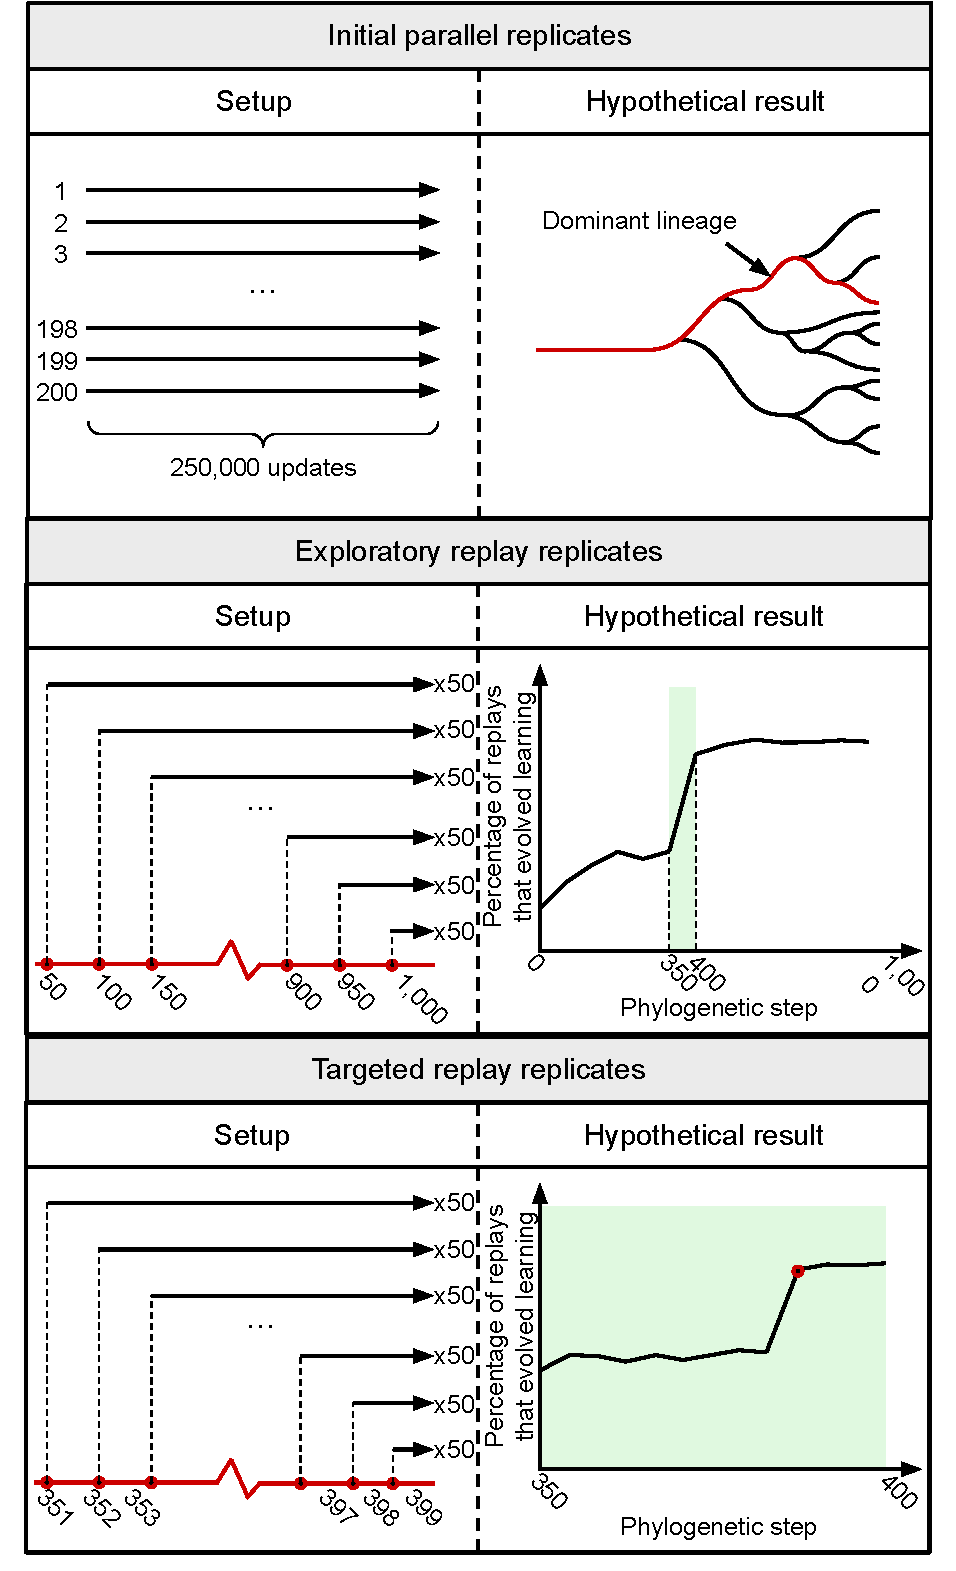
\includegraphics[width=0.65\textwidth]{03_learning_case_studies/media/conceptual_figure.pdf}
\caption{
    Illustration of the experimental design and hypothetical results.
    The top panes show the 200 initial parallel replicates seeded with the ancestral genotype and evolved for 250,000 updates.
    We extracted the lineage of the most abundant genotype in the evolved population (the dominant lineage), shown in red. 
    %When these replicates finish, we can classify each replicate and extract the dominant lineage (in red) from the phylogeny.
    Next, we conducted exploratory replays (middle panes) by launching replay replicates at regular intervals along focal lineages. 
    These exploratory replays give a coarse-grained view of how potentiation changed over a lineage. 
    We identified the window with the largest potentiation gain, shown as the shaded region.
    Finally, we ran targeted replay replicates for every step in this potentiation window. 
    %Phase 2 takes each dominant lineage from Phase 1 and launches replay experiments every 50 steps along the lineage. 
    %An example potentiation graph is shown, where a substantial increase in potentiation occurs between steps 350 and 400. 
    %We then seed \textit{additional} replay replicates for Phase 3, one for each step in the window identified in Phase 2.
    These fine-grained replay replicates show mutations that resulted in large potentiation increases (shown here with a red dot). 
}
\label{fig-conceptual}
\end{center}
\end{figure}

% Introduce three-phase design and give a brief overview of each part
To identify mutations that substantially increased the likelihood that learning evolved, we split the work into three phases (see Figure \ref{fig-conceptual} for an overview).
%
First, we seeded 200 initial parallel replicates in the associative learning environment with a default ancestor only capable of reproduction. 
Each replicate was given 250,000 updates, where one update is the time it takes for all organisms to execute 30 instructions, on average. 
% These replicates evolved for 250,000 updates, where one update is the
% and evolved them for 250,000 updates.
%For each of the 200 replicates, 
We identified the most abundant genotype in each final population to represent the replicate and classified its behavior. 
%By tracking the phylogeny in each replicate, 
We then extracted the ``dominant lineage'', stretching from the ancestor to the representative genotype. 
%(i.e., the \textit{dominant genotype} of that replicate), classified its behavior, and extracted its lineage from the ancestor. 
Each step in the lineage corresponds to a change in genotype between parent and offspring, with clonal offspring occupying the same step as their parent.
While a step is often a single mutation, it is possible that one step is composed of multiple co-occurring mutations.

To begin analyzing changes in potentiation, we ran exploratory replays replicates on four lineages capable of learning.
%Due to the computational cost of these replay experiments, we performed replays on only four learning replicates.
For each, we seeded independent replicates for every $50^{th}$ step in the lineage, up to step 1,000.
All replay replicates evolved in the same associative learning environment, and replays were given the same number of updates as had %equal to the number of updates that 
occurred after that genotype first appeared (e.g., replays for a genotype that appeared at update 150,000 would be evolved for the remaining 100,000 updates). 
Potentiation was measured as the portion of replay replicates that evolved learning. % divided by the number of replay replicates that finished. 
Because replays were seeded with a single organism, some replay populations went extinct before ever reproducing and thus were not factored in (the minimum number of finished replay replicates from a given lineage step was 38, while three case study lineages had a minimum of 48). 

While the exploratory replays provide an overview of how potentiation changed, we dug deeper by running targeted replays to further explore windows of increasing potentiation.
Specifically, we found the 50- or 100-step ``potentiation window'' that sees the largest increase in potentiation in the exploratory results, and seeded additional replays for every step in that range.
These targeted replays were conducted identically to the exploratory replays, only they did not skip steps.
Though computationally expensive, these replays illuminated the impact every genotypic change had on potentiation. 
Running 50 replay replicates per step still results in considerable noise, but we were able to identify mutations that clearly and substantially increased potentiation using these targeted replays.

We hand-analyzed algorithms in all potentiating mutations, here defined as single lineage steps that result in a potentiation increase of 25 percentage points or more.
%These potentiating mutations and other steps around them in the lineages were hand-analyzed to understand the underlying algorithm encoded in each genotype and how changes to that algorithm may have potentiated the lineage. 
Further, we assessed genotype fitness in context of their lineage to identify if potentiation mutations were beneficial, deleterious, or neutral. 
Finally, %mutation analyses were conducted to 
we characterized the local fitness landscape of each genotype (one and two mutations out), measuring the presence and fitness of nearby genotypes capable of learning. 
%All two-step mutations were analyzed for each potentiating step and the step before it, to investigate whether the potentiating step increased the presence of learning in the local landscape, increased the benefit of learning, etc. 

% We then took four lineages that exhibited learning and performed exploratory replays.
% These exploratory replays took the learning lineages and conducted a ``coarse-grained'' sampling of the lineage via analytical replay experiments. 
% We ran replay replicates for every 50 steps along the lineage, out to step 1,000. 
% This provided a window into how the likelihood of evolving learning changed over time.%, and importantly, identified any periods of substantial increases in that likelihood. 
% Finally, in we isolated these period(s) of drastic increases in likelihood and ran additional targeted replay replicates in that window (one for each step along the lineage). 
% This would then show us the impact of individual steps along the lineage, potentially highlighting single steps with massive changes in potentiation. 

% % What did our replay experiments look like?
% %\subsubsection{Analytical replay experiments}
% %After identifying the replicates that evolved learning, we can then begin to analyze their evolutionary history. 
% %We tracked phylogenetic data on all extant organisms and their ancestors, so we can trace a line of descent from the final dominant genotype to the original ancestor. 
% %After identifying the replicates that evolved learning, we then started analytical replay experiments.
% %For each learning replicate, we seeded \textit{additional} evolutionary runs along the dominant genotype's lineage. 
% %Lineages are based on genotypes, so each ``step'' corresponds to a reproduction event where one or more new mutations were introduced in the new offspring. 
% %Starting at step 50, we seeded 50 replay experiments at every $50^{\text{th}}$ step up through step 1,000. 

% %Replay replicates evolved to match the 250,000 updates of the initial replicates.
% %Replays starting from early points in the lineage thus saw more new updates than replays from points farther along the lineage. 
% %As an example, if a replay starts from step 200 and the genotype was first seen at update 100,000, we would run the replicates for step 200 for 150,000 updates. 
% %These evenly-spaced replay replicates were than manually inspected for any large jumps in potentiation. 
% %If evidence of large jumps was detected, we then seeded fine-grained replay replicates for every step between the two multiples of 50.

% % \subsubsection{Initial parallel replicates}

% % % General info, 200 reps for 250k updates starting with a default ancestor
% % We stared by founding 200 parallel replicates (see top panels of Figure \ref{fig-conceptual}). 
% % Each replicate started with one organism: the ancestor organism, which consists of 99 no-operation instructions and 1 \texttt{Repro} instruction. 
% % This organism only reproduces itself, it does not interact with the environment and thus cannot receive any rewards or punishment. 
% % Each replicate was given 250,000 updates, where one update is the time it takes for all organisms to execute 30 instructions, on average. 
% % All replicates ran in the same associative learning environment.

% % % Phylogeny tracking and isolating the final dominant genotype + lineage 
% % % CITE Emily? 
% % We tracked pruned genotypic phylogenies for these initial replicates. 
% % Digital evolution has the advantage of perfectly tracking all reproduction events and storing parent-child relationships. 
% % To reduce the storage overhead, we pruned the phylogenies to only track the extant population and any ancestors of those organisms. 
% % In the end, this gave us the lineage from the ancestral organism to any genotype in the extant population at the end of the 250,000 updates. 
% % As a representative of the final extant population, we extracted the most abundant extant genotype (i.e., the dominant genotype of that replicate) and isolated its lineage.



% \subsubsection{Exploratory replay replicates}

% After the initial parallel replicates concluded, we had a set of replicates that had evolved and maintained associative learning at the end of 250,000 updates. 
% Since we know learning evolved along each of these lineages, we are interested in how the \textit{potentiation} for learning changed along the lineages (i.e., at what points along the lineage was lineage more likely to appear than not, and where did the largest jumps in potentiation occur?).
% To investigate these changes in potentiation, we took a subset of these replicates and conducted a batch of coarse-grained replay experiments to look for large gains in potentiation while conserving computational resources.
% For a given lineage, we seeded 50 replay populations at every $50^{th}$ step along the lineage (see the middle panes of Figure \ref{fig-conceptual}.
% Regardless of the length of the lineage, we stopped at step 1,000, only continuing beyond that point if the potentiation had not approached 100\%.

% To measure potentiation at a point along the lineage, we ran the 50 replay replicates and then calculated the percentage of those replicates that evolved learning (e.g., if 30 replays out of 50 evolved learning, that point would have a potentiation of 60\%). 
% These exploratory replay replicates gave us a summary of how potentiation changed over the course of the lineage. 
% More specifically, we could look for windows containing large potentiation increases. 
% If single mutations conferred large jumps in potentiation, we would expect them to occur in windows of substantial potentiation gain.
% Since all lineages started from the same ancestor, the results from the initial parallel replicates were used for step 0 of every lineage to save computational power.

% \subsubsection{Targeted replay replicates}

% Once the exploratory replays were conducted, we had a summary of how the potentiation changed over the course of the lineage. 
% We used this exploratory replays to identify periods of drastic potentiation gain. 
% The exploratory replays occurred at every 50 steps along the lineage, so we identified the 50-step window that resulted in the greatest increase in potentiation (and for the first two lineages we took a 100-step window as to maximize our chances of finding mutations that confer large jumps in potentiation. 

% Once the target window was identified, we repeated the process of running replay experiments. 
% This time we seeded replays from every step along the lineage inside the target window. 
% While computationally expensive, this illuminates the impact every change in genotype had on potentiation. 
% While 50 replay replicates per lineage step still results in considerable variation, we were able to identify mutations that clearly and substantially increased potentiation using these targeted replays. 

% Once a potentiating step was identified, we analyzed various aspects of the genotype and the evolutionary characteristics surrounding it. 
% These potentiating steps and other steps around them in the lineages were hand-analyzed to understand the underlying algorithm encoded in each genotype and how changes to that algorithm may have potentiated the lineage. 
% Further, the genotypes were assessed in context of the lineage to identify if these potentiation events were beneficial, deleterious, or neutral in terms of fitness. 
% Finally, mutation analyses were conducted to characterize the local fitness landscape and its relationship to learning. 
% All two-step mutations were analyzed for each potentiating step and the step before it, to investigate whether the potentiating step increased the presence of learning in the local landscape, increased the benefit of learning, etc. 

% % How did we conduct our mutational analysis?
% %\subsubsection{Mutational landscape analysis}

% Not sure if we'll have real statistics, but we'll definitely have data to upload
\subsection{Data and software availability}

Both the data and the software used to conduct this work are available in the supplemental material \citep{fergusonFergusonAJReplayingEvolution2023}.
Analyses were conducted in the R statistical computing language \citep{r_core_team_r_v4} using the \textit{dplyr} package to summarize data \citep{wickhamDplyrGrammarData2022}.
Data was visualized using the \textit{ggplot2} and \textit{cowplot} packages \citep{R-ggplot2, R-cowplot}.

\section{Results}

Here we discuss the generation and analysis of the initial replicate runs, followed by the more detailed results from each of the four case study lineages.

\begin{figure}[!h]
\begin{center}
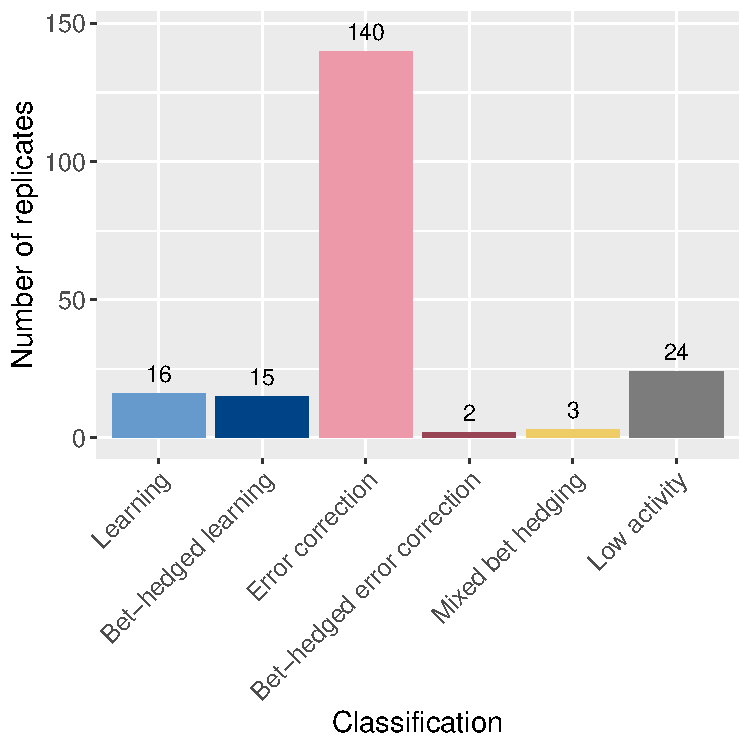
\includegraphics[width=0.65\textwidth]{03_learning_case_studies/media/final_dom_classification.pdf}
\caption{Behavior classification of the final dominant genotypes from the 200 initial parallel replicates.}
\label{fig-final-dom-classification}
\end{center}
\end{figure}

% \begin{figure}[t]
% \begin{center}
% 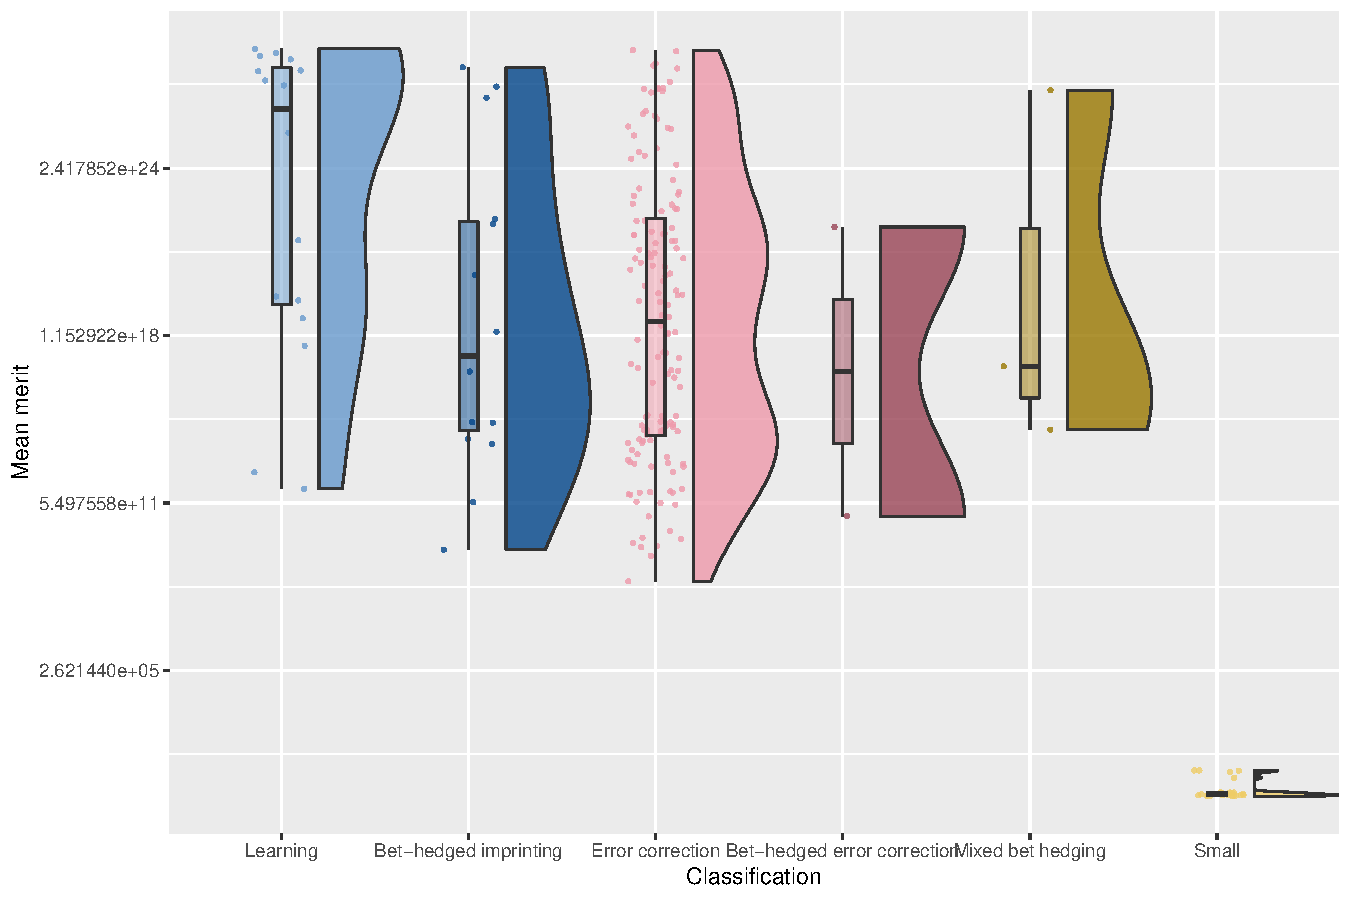
\includegraphics[width=0.45\textwidth]{media/raincloud_rep_merit.pdf}
% \caption{TODO}
% \label{fig-final-dom-rep-merit}
% \end{center}
% \end{figure}

\vspace*{-10mm}

\subsection{Evolution of learning in the initial replicates}
In the first phase of this study, we evolved 200 independent replicates for 250,000 updates (about 3600 generations) in the associative learning domain, each starting with a default ancestor. % capable only of self-replication.
%This setup allowed populations to experience approximately 3600 generations; 
The distribution of evolved behaviors is shown in Figure \ref{fig-final-dom-classification}.
Only 16 of 200 replicates exhibited associative learning.
An additional 15 replicates evolved forms of bet-hedged learning, with two of those replicates gaining and then losing associative learning along their lineage.
The majority of replicates relied on some form of error correction, either as a sole strategy (140), a bet-hedged variant (2), or as a fallback due to limited learning (3). 
%Both bet-hedged error correction replicates have a subset of environments that caused them to fall into cycles of repeatedly choosing the wrong action.%choosing the wrong action, backing up, and then choosing the same wrong action. 
%This prevented them from gaining any additional fitness. 
%Of the three mixed bet-hedging replicates, one exhibited learning in one environment and error correction in the other three
%The other two replicates exhibited the same behavior in all environments: a pseudo-learning strategy that failed on certain sequences of cues and fell back on error correction too often to hit the 90\% accuracy required to be classified as learning.
Finally, 24 replicates failed to navigate enough states to categorize them, leading us to label them as ``low activity''. 

We analyzed all 16 replicates that evolved and maintained learning, identifying the length of their lineages from onset of evolution until learning stabilized, no longer showing further improvement.
Given the substantial computational power required for each time point studied, we performed replay experiments only on the shortest three such lineages (lineages A-C), plus the shortest lineage that exhibited error correction at some point in its evolutionary history (lineage D).
%Of the 16 replicates that evolved and maintained learning, we performed replay experiments on four of them.
%The first three replicates were selected for having the shortest number of steps along a lineage before fitness stopped increasing. 
%The fourth was selected for the same reason, but was selected from among the four replicates that contained error correction in their lineages. 
%These replicates were selected to save computational resources.
%The number of updates experienced by a replay replicate was calculated as the number of updates between the genotype's first appearance in the population and the 250,000 update limit for the initial replicates. 
%Thus longer lineages A) have the potential to require more exploratory replays before saturating to $>90$\% potentiation and B) typically require more updates per replay for early steps in the lineage. 
Selecting these particular replicates to replay has the potential to bias the results, as discussed below.

% \begin{table}[!t]
% \centering
%     {\rowcolors{2}{white}{lightgray!20}
%     \begin{tabular}{ |c|c|c|c|c| }
%         \hline
% %        \makecell{Lineage} & \makecell{Initial \\ seed} & \makecell{Potentiating \\ mutation depth} & \makecell{Potentiation \\ increase} & \makecell{Fitness \\ effect} &  \makecell{Steps before \\ learning} & \makecell{Percentage of \\ updates persisted} \\
%         % \makecell{Lineage} & \makecell{Initial \\ seed} & \makecell{Potentiating \\ mutation depth} & \makecell{Potentiation \\ increase} & \makecell{Fitness \\ effect} &  \makecell{Steps before \\ learning} & \makecell{Potentiating \\ mutation persistence} \\
%         % \hline
%         % A & 86 & 484 & 58pp & Neutral & 53 & 89\% \\ 
%         % B & 4 & 104 & 36pp & Beneficial & 91 & 100\% \\ %1096 (all) \\ 
%         % C & 15 & 279 & 64pp & Deleterious & 26 & 100\% \\ %1978 (all) \\ 
%         % D & 6 & 548 & 50pp & Neutral & 8 & 100\% \\ %589 (all) \\ 
%         \makecell{Lineage} & \makecell{ mutation \\ depth} & \makecell{Potent. \\ increase} & \makecell{Fitness \\ effect} &  \makecell{Steps to \\ learning} \\
%         \hline
%         A & 484 & 58pp & Neutral & 53 \\ 
%         B & 104 & 36pp & $+$ & 91 \\ %1096 (all) \\ 
%         C & 279 & 64pp & $-$ & 26 \\ %1978 (all) \\ 
%         D & 548 & 50pp & Neutral & 8 \\ %589 (all) \\ 

%         \hline
%     \end{tabular}
%     \caption{
%     Summary of targeted replay traits.
%     }
%     \label{tab:replay-summary}
%     }
% \end{table}



\subsection{Case studies of individual lineages}

\begin{figure*}[!th]
    \begin{center}
    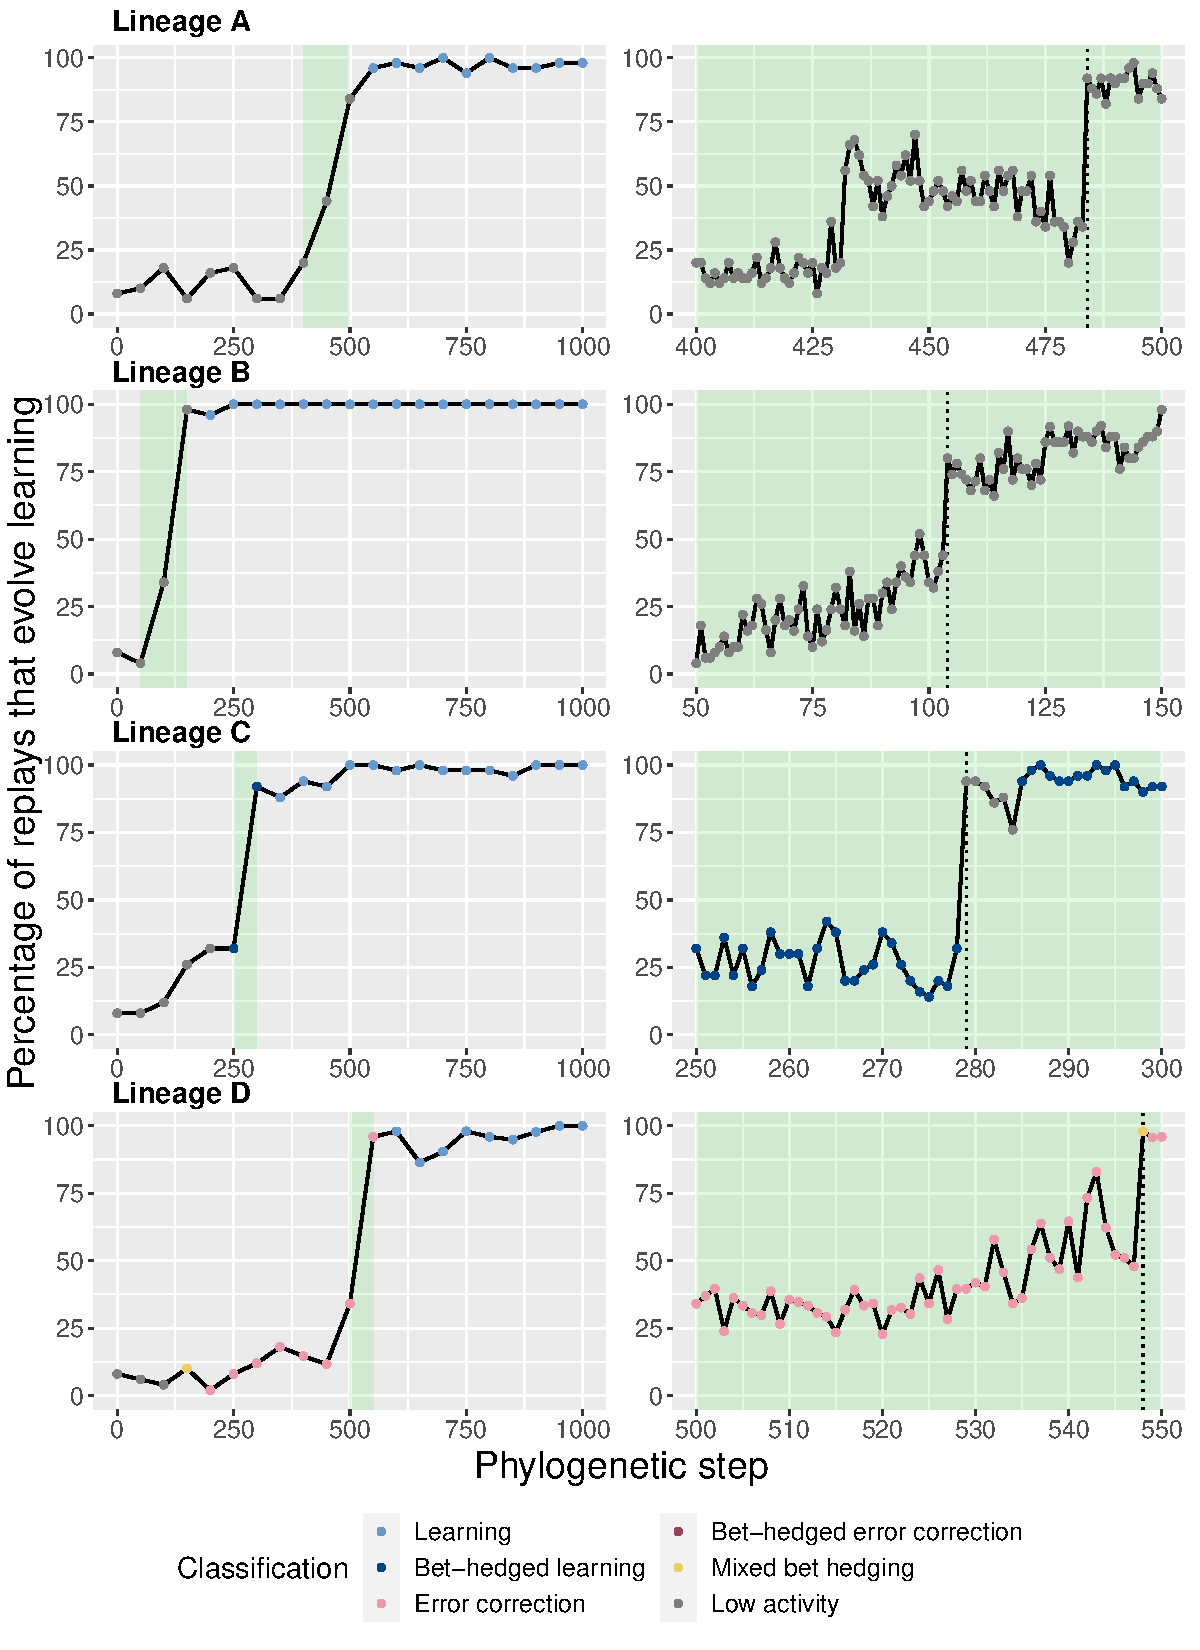
\includegraphics[width=0.8\textwidth]{03_learning_case_studies/media/combined_replays_R.pdf}
    \vspace*{-3mm}
    \caption{
        Potentiation of associative learning for all case studies, shown as the percentage of replicates that evolve associative learning when replayed from a given genotype. %evolution is replayed starting at that point. %, as it changes over the lineage for the four case studies. 
        For each case study, the left plot shows the results of the exploratory replays. 
        We identified a window of potentiation gain in each lineage, indicated by the shaded region. 
        Within that window, we conducted targeted replays for every step along the lineage, shown on the right. 
        %The results of those targeted replays are shown in the plots on the right.
        The color of the points corresponds to the behavior exhibited at that step of the lineage. 
        A dotted line in the targeted replays indicates the step that conferred the most potentiation.
    }
    \label{fig-potentiation-all-case-studies}
    \end{center}
\end{figure*}

Below we present the results of the replay experiments performed on the four focal lineages and provide a step-by-step analysis of how key mutations altered both immediate fitness and evolutionary potential (potentiation).
Where possible, we explained how these mutations altered the underlying algorithms.
For each lineage, potentiation across both exploratory and targeted replays can be found in Figure \ref{fig-potentiation-all-case-studies}.
%Additionally, details about the most-potentiating mutation from each lineage can be found in Table \ref{tab:replay-summary}.

\subsubsection{Lineage A}

% \begin{figure}[!h]
%     \begin{center}
%     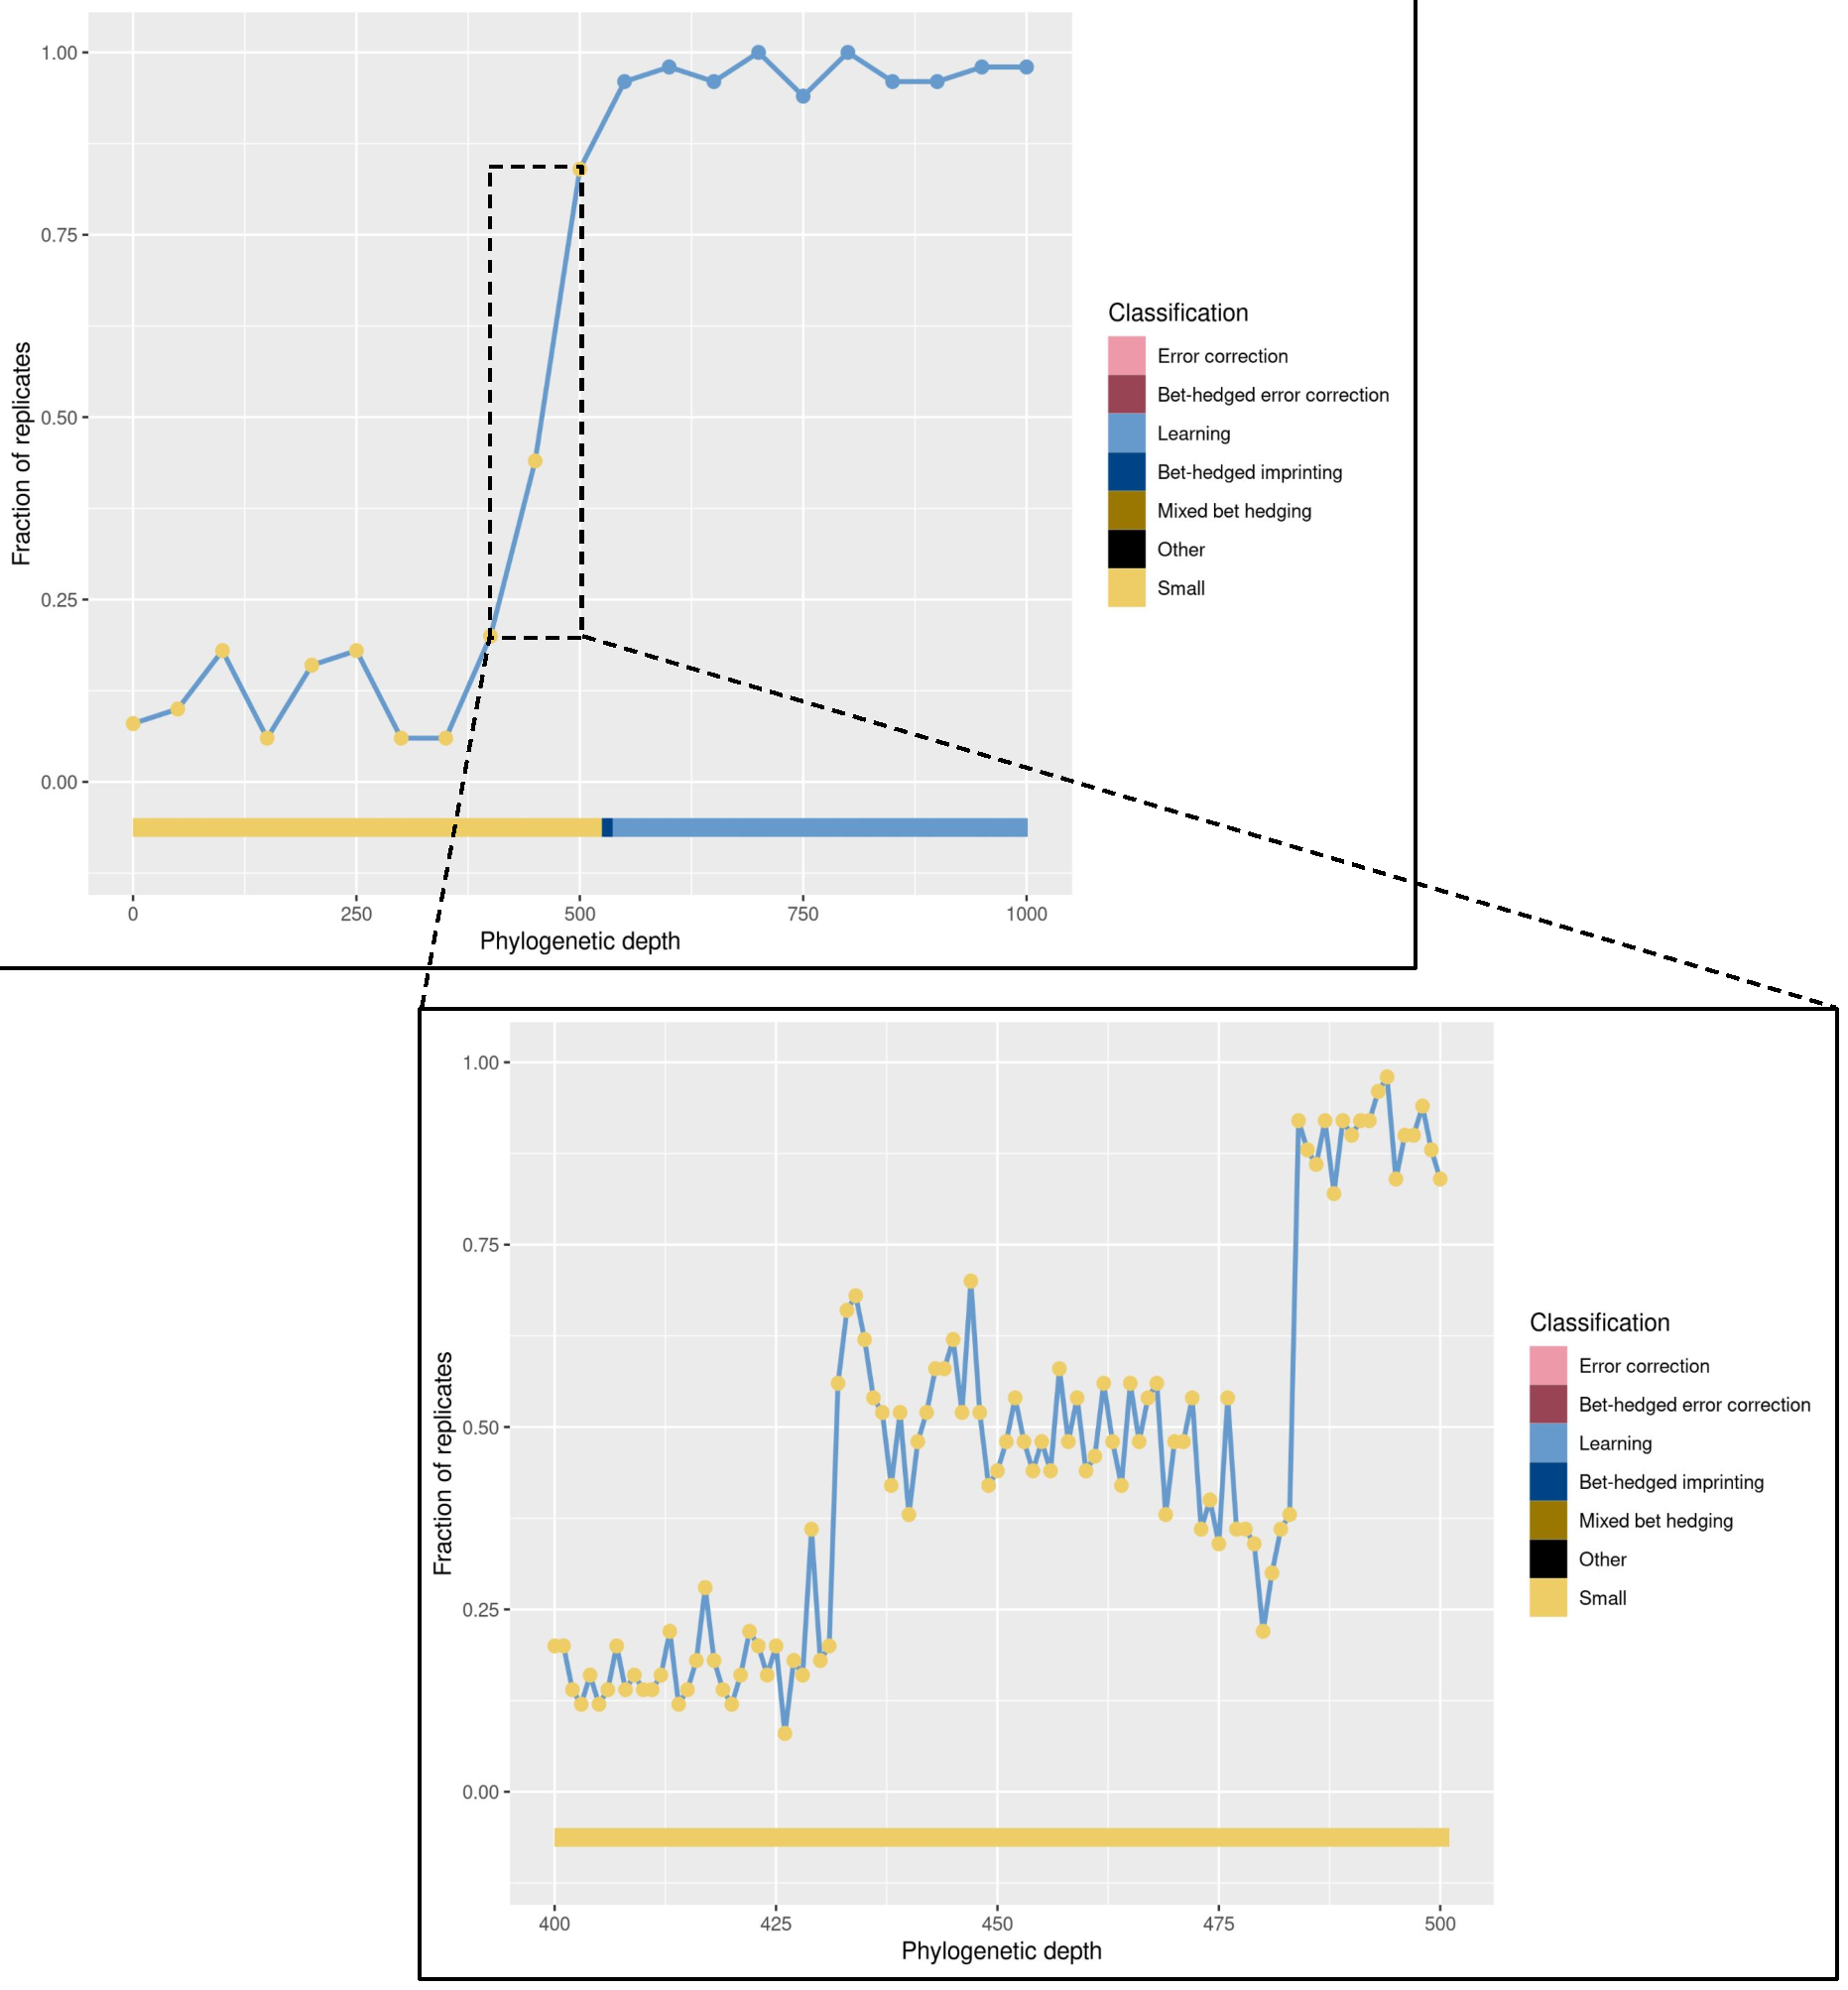
\includegraphics[width=0.45\textwidth]{media/test_pop_out_seed_86.pdf}
%     \caption{
%         \textbf{Case Study A}.
%         Potentiation of associative learning, shown as the fraction of replicates that evolve associative learning when replays are started at that point, as it changes over the lineage for Case Study A. 
%         The top figure plot shows the results of the exploratory replays. 
%         Two windows of increased potentiation were identified, indicated by the dashed rectangle. 
%         Results of the targeted replays are shown in the bottom, pop-out plot.
%         Both lines and points show potentiation at various steps along the lineage. 
%         The color of the points corresponds to the behavior exhibited at that step of the lineage.
%         The rectangle at the bottom of the plot also shows the behavior at the lineage, but with more detail than the evenly spaced points of the exploratory replay.
%     }
%     \label{fig-potentiation-case-study-a}
%     \end{center}
% \end{figure}

Our first case study is one of the shortest lineages and it contains a quick jump to learning (at step 537) from low activity, with only a brief time spent in bet-hedged learning. 
%The exploratory and targeted replays for Case Study A are both shown in Figure \ref{fig-potentiation-case-study-a}.
Exploratory replays for this lineage revealed a stark jump in potentiation between 400 and 500 steps from the ancestor, which we call the potentiation window.
From step 400 to step 450, potentiation increased from 20\% of replicates to 44\%, and increased again to 84\% of replicates by step 500. 
Before this window, potentiation fluctuated around the original 8\% found starting from the default ancestor.
%Before this jump, the potentiation fluctuates between 6\% of replicates and 20\% of replicates evolving learning. 
After the selected window, potentiation increased once more and then fluctuated between 94\% and 100\%. 

With this in mind, we seeded 50 replays for each genotype in the potentiation window. 
%Since we run 50 replicates at each step, there is considerable noise in the data. 
%Regardless, two mutations confer drastic increases in potentiation: steps 432 and 484. 
Even with the noise due to a small sample size, %that comes from having only 50 replays at each step,
we identified two mutations that conferred sizable increases in potentiation: steps 432 and 484.
The mutation at step 432 brought potentiation above 50\% for the first observed time in the lineage. 
Surprisingly, potentiation then decreased (on average) back to a local minimum of 20\% of replicates at step 480. 
Finally, the mutation at step 484 substantially increased potentiation to 92\%, where it stayed for all subsequent replays. 
%Looking at performance averaged over 100 trials, both mutations are neutral in fitness.

Even though the largest jump in potentiation occurred at step 484, learning did not appear in the lineage until step 537. 
That said, only steps 516 and 525 caused any change in behavior; all other interim mutations occurred in unexecuted regions of the genome. 
The potentiating mutation at step 484 made a key instruction in the main loop of the genome redundant.
It had no immediate effect on fitness, but later (in intermediate step 516) allowed the redundant instruction to be replaced by
%, mutating the redundant instruction into 
a right turn that granted a small fitness increase as organisms could now navigate until they reached the second left turn. 
Step 525 further improved navigation, but used a comparison that made an unfounded assumption on whether the left or right random cue is larger. 
When the assumption was correct organisms were capable of learning the cues, however the assumption is only correct 50\% of the time, so this genotype is categorized as bet-hedged learning. 
Finally, step 537 swapped that comparison with one that makes no assumptions about cue values, enabling the genotype to learn in all environments. %and now the genotype can always learn. 

Looking at the local mutational neighborhood, the potentiating mutation at step 484 increased the number of two-step mutations that conferred learning from 2 to 9 (of approximately 56 million). 
Additionally, the fitness of the learning mutations in the local neighborhood increased by three or four orders of magnitude.
%Specifically, the mutation at step 484 adds a \texttt{Decrement} instruction at the very first position in the genome. 
%This makes another \texttt{Decrement} instruction in the midst of the main section of the genome obsolete, as it was only called once and now is never called because of the new mutation. 
%With that locus now free to mutate, step 516 sees a mutation at that exact locus, swapping it to a \texttt{Right} movement instruction.
%This allows organisms to move right for the first time, which they do successfully a few times before being stumped by a \textit{left} immediately followed by a \textit{right}.
%Finally, the mutation to learning at step 537 adds more flow control before the new \texttt{Right} instruction, alleviating the issue and allowing organisms to cleanly handle any sequence of states. 
%These three mutations saw a shift from less than 7 correct states, on average, at step 484, to less than 10 at step 516, to over 115 at step 537, resulting in a drastic fitness increase.
%While was purely neutral in fitness when it occurred, the mutation at step 484 shifted the genetic material to allow changes to the vital machinery and paving the way for learning. 

What about the earlier potentiation that was gained and then lost?
The mutation that substantially increased potentiation at step 432  introduced a comparison that had no immediate fitness effect. 
This comparison remained unimportant until step 525 when it became integral in introducing bet-hedged learning. %interacted with that new comparison to improve the algorithm. 
%Looking at two-step mutations, neither step 432 nor the step before had any learning in their local landscapes. 
Neither step 432 nor its predecessor had access to learning within a two-step mutational range.
Thus, it is likely that the potentiation comes from that comparison given that we observed it being utilized for learning later on.

%The earlier potentiation at step 432 swapped a \texttt{Push} instruction for an \texttt{IfLess} instruction. 
%At the time, this did nothing. 
%In fact, this instruction only comes into play at step 537, where it becomes part of the logic of ``if B does not equal C AND C is greater than or equal to 3, then take a right turn''. 
%Thus, while it took a while to get there, the mutation was directly useful in the learning algorithm. 

%[MOVE TO DISCUSSION???]
Why then, did potentiation decrease between steps 432 and 484?
At step 432 (and indeed before it), the algorithm had a section where if register B was non-zero, then B stored the cue associated with a left turn. 
While this information was likely to make the evolution of learning easier, it was unused at that time. 
As such, the mutations between steps 432 and 484 dismantled that machinery, requiring a replacement to be built before learning could evolve.

%increasing the number of mutations needed for learning to evolve. 
%Indeed, this machinery was rebuilt before learning evolved, but in a different way. 

\subsubsection{Lineage B}

% \begin{figure}[!h]
% \begin{center}
% 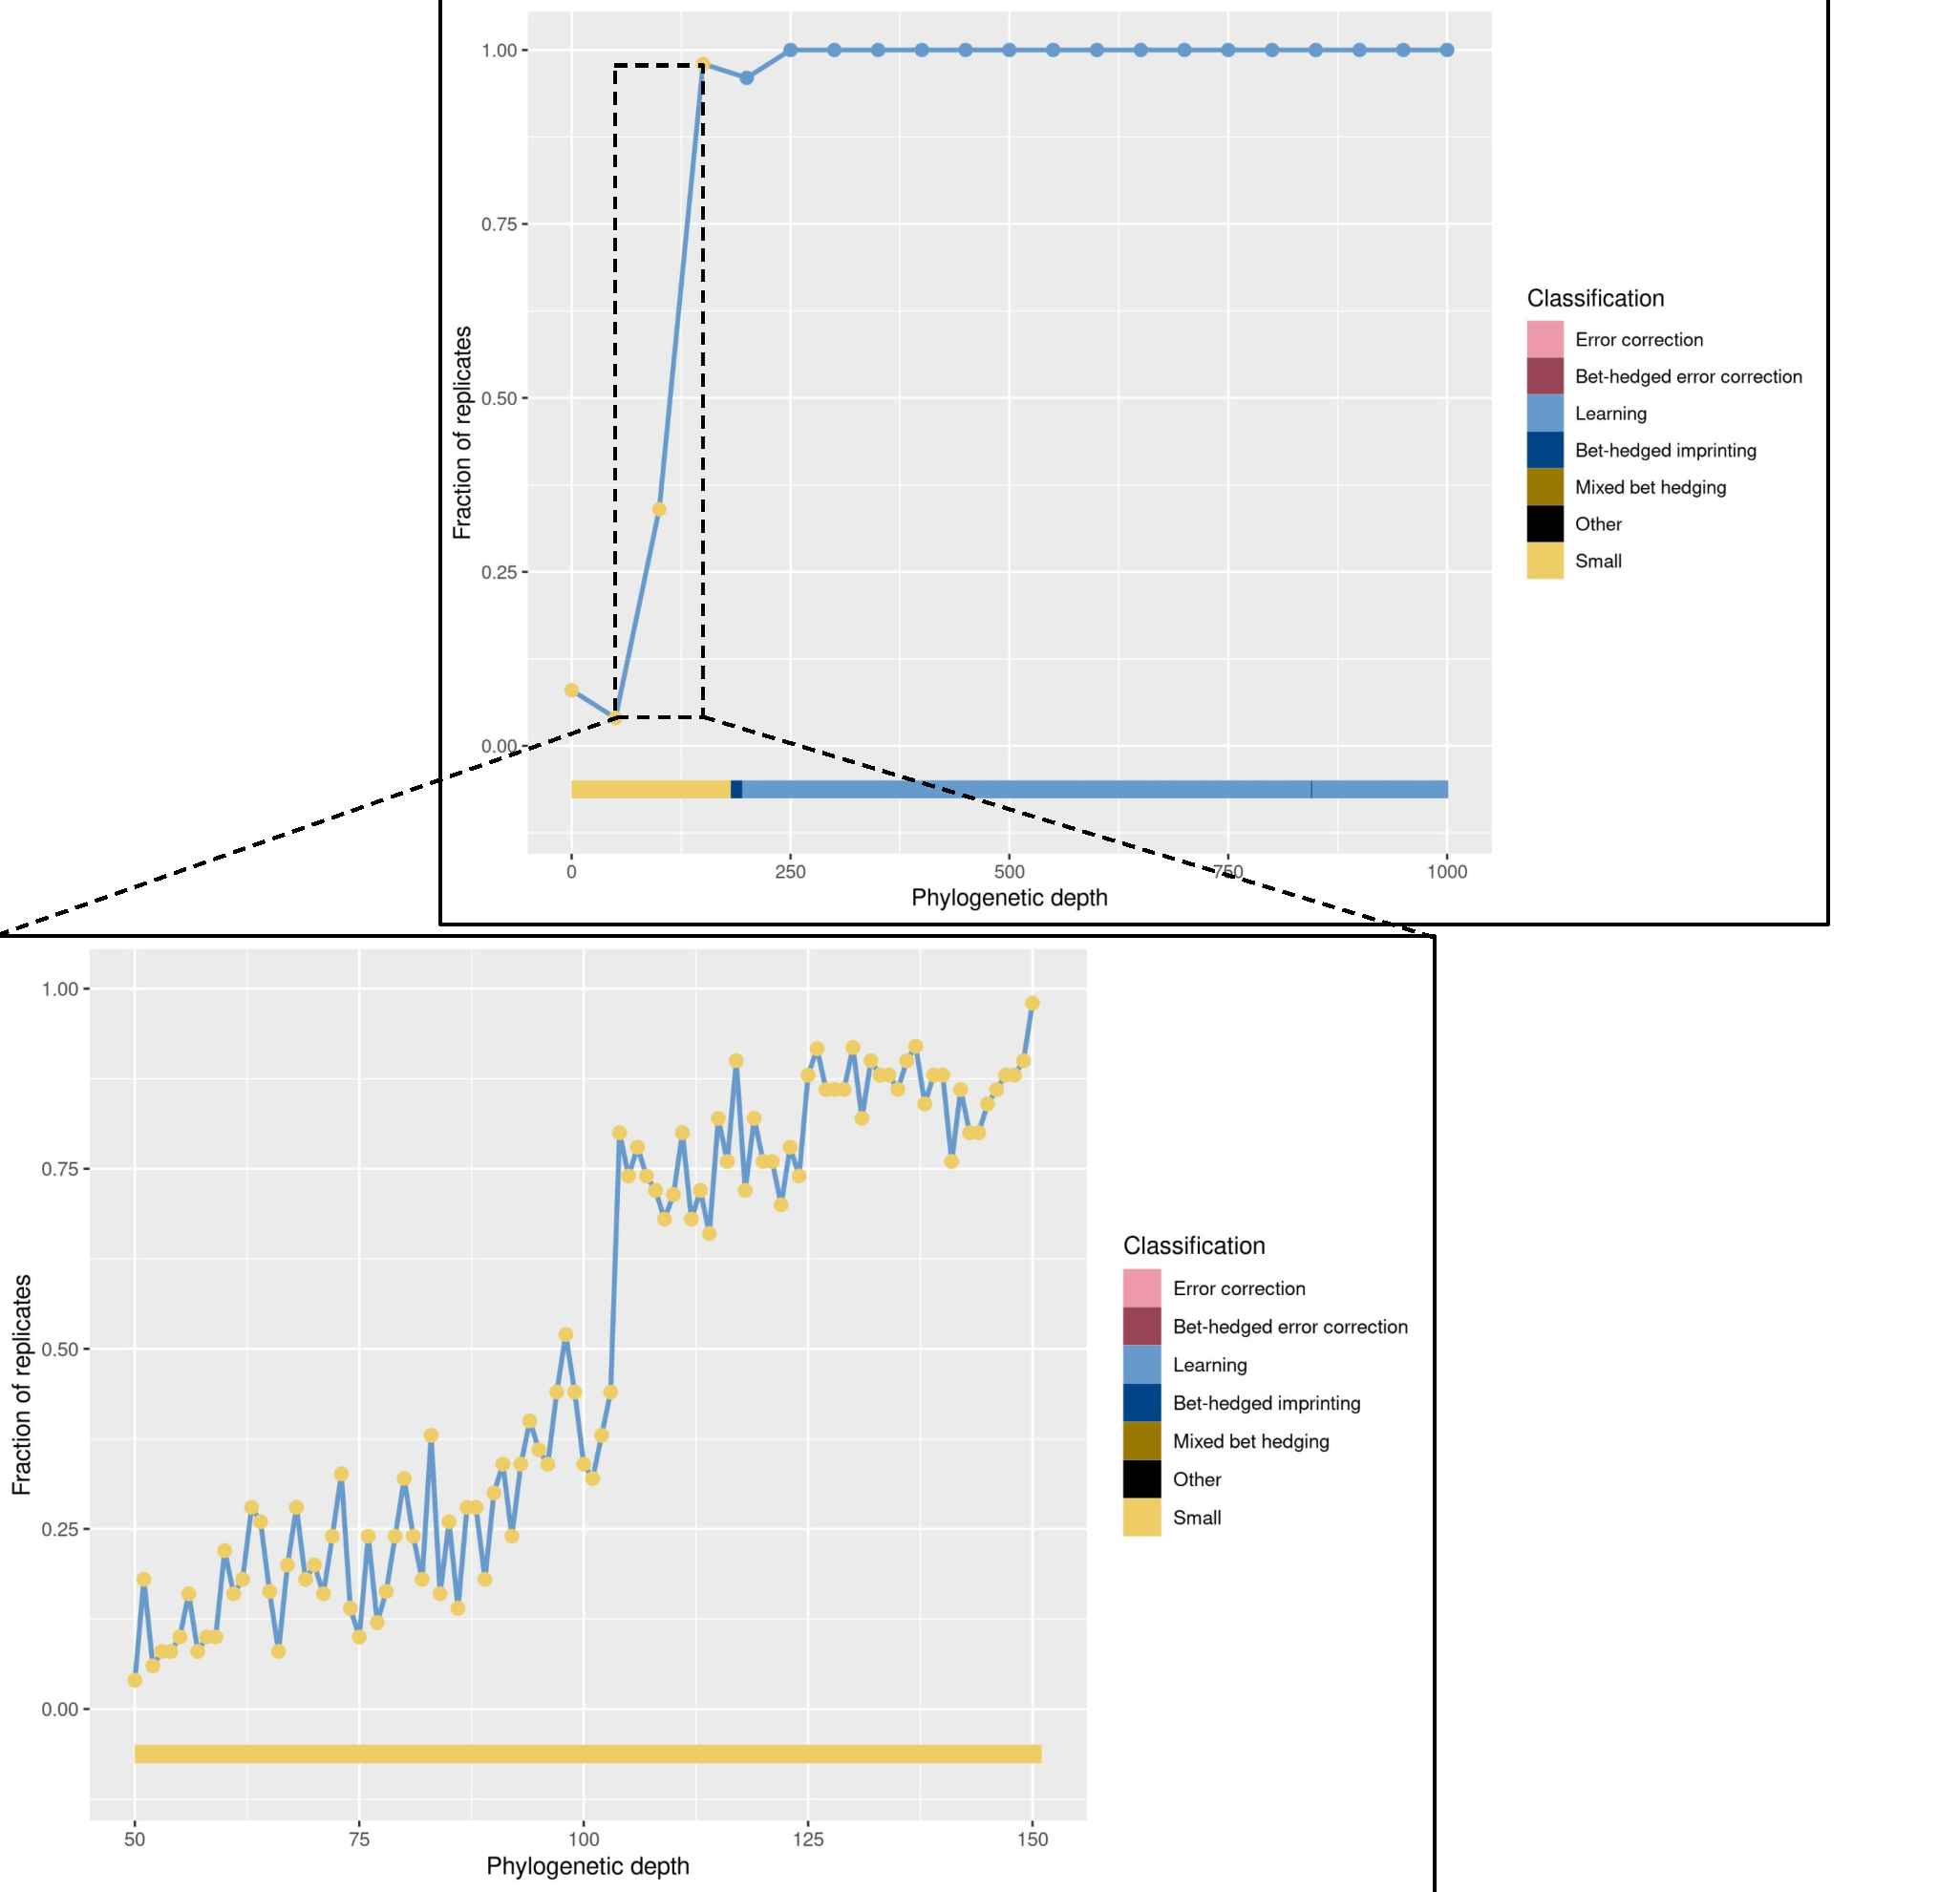
\includegraphics[width=0.45\textwidth]{media/test_pop_out_seed_4.pdf}
% \caption{
% \textbf{Case Study B}.
% Potentiation of associative learning as it changes over the lineage for Case Study B. 
% The top figure plot shows the results of the exploratory replays. 
% Two windows of increased potentiation were identified, indicated by the dashed rectangle. 
% Results of the targeted replays are shown in the bottom, pop-out plot.
% Both lines and points show potentiation at various steps along the lineage. 
% The color of the points corresponds to the behavior exhibited at that step of the lineage.
% The rectangle at the bottom of the plot also shows the behavior at the lineage, but with more detail than the evenly spaced points of the exploratory replay.}
% \label{fig-potentiation-case-study-b}
% \end{center}
% \end{figure}

Similar to Lineage A, this lineage transitioned from low activity to learning through a brief period of bet-hedged learning. 
Exploratory replays on this lineage reveal that learning was potentiated almost immediately; by step 150 potentiation had climbed above 95\%, where it stayed for the rest of the lineage. 
%From this exploration we identified 
As such, the potentiation window included steps 50 through 150. %, and therefore targeted that windows for additional replays. 

Unlike Lineage A, the targeted replays reveal a general trend of increasing potentiation, with step 104 as a notable outlier. 
%However, one mutation stands out as an outlier: step 104. 
Mutations from steps 50 through 103 slowly increased potentiation from 4\% to 44\%, but the mutation at step 104 jumped to 80\%. 
From there, another slow increase continued to raise potentiation to a peak of 98\% at step 150.

Learning did not appear until step 195, over 90 steps beyond the largest potentiating mutation. 
Given that 34 intermediate mutations altered the encoded algorithm, the mechanistic pathway to achieve learning is more complicated than can be broken down in this work.
%breaking down the exact details of the changes to reach learning is beyond the scope of this work. 
However, the potentiating mutation at step 104 modified the execution flow of the genome, which appears to have been essential for the later evolution of learning. % in the long term. 

While two mutations occurred at step 104, only one caused a functional change: an instruction to swap data between registers was mutated to a left turn. 
Prior to this mutation, the genome encoded a left turn later on, after which the execution became trapped in an endless loop. 
The potentiating mutation was immediately beneficial; it allowed organisms to take the left turn earlier, which, in turn, allowed them to avoid the loop. 
%As such, this mutation was immediately beneficial when it occurred.
As a side effect, a large portion of the genome that was previously executed was now skipped, and these instructions remained skipped when learning evolved 91 steps later.
%In avoiding the infinite loop, a large portion of the genome was now skipped and remained so when learning evolved 91 steps later. 
Looking at the local fitness landscape, learning was neither present in the potentiating step's landscape nor in the step before.
We hypothesize that the potentiation came from the change in execution flow, and that skipping over those instructions avoided a pitfall and freed up execution time that may have been useful in evolving learning.

%While two mutations occurred at step 104, only one provides a functional change. 
%That mutation is a point mutation swapping a \texttt{Swap} instruction for a \texttt{Left} movement instruction. 
%Another \texttt{Left} instruction already existed a little further along the genome, but removing the \texttt{Swap} instruction allowed execution to jump back to the main portion of the genome, while still executing the needed left turn before doing so. 
%This increased fitness immediately, as it prevented the organism from getting stuck in an infinite loop at toward the end of the genome, instead correctly handling a few more states. 
%Secondly, this caused a large portion of the genome to not be executed, most of which is still skipped when learning evolved at step 195. 
%The mutation at step 104 did prove important, as it persisted throughout evolution, being present in the final genome at step 1544.


\subsubsection{Lineage C}

Lineage C has the biggest single-mutation potentiation increase (64 percentage points), and that mutation was deleterious when it occurred at step 279 along the lineage.  
Learning later appeared at step 305. 

The potentiating step mutated a no-operation instruction into a conditional flow control instruction. 
%On the existing genetic background, this mutation was terrible for fitness.
At step 278 the genotype was capable of bet-hedged learning, but the mutation at 279 knocked out all instances of learning, reclassifying the behavior as ``low activity.'' %down below the classification threshold. 
The next step restored some fitness, and then step 285 interacted with the mutation at 279 to not only restore fitness, but to dramatically improve it. 
Ultimately, the potentiating mutation at step 279 allowed the algorithm to more precisely discriminate between the left and right cues. 
%Prior to the mutation, a less-than comparison was used, which only functioned correctly in instances where the \textit{left} cue was less than the \textit{right} cue; this assumption was only valid half the time, resulting in the bet-hedged learning seen before the potentiating mutation. %left the algorithm at the mercy of the random cue values. 
Prior to the mutation, a less-than comparison was used, which only functioned correctly in 50\% of instances, specifically those where the \textit{left} cue was less than the \textit{right} cue. 
%This assumption resulted in the bet-hedged learning seen before the potentiating mutation.
%The potentiating mutation switched it to an equality comparison, which alleviated the assumption and paved the way for learning in all instances. %that one cue will be larger than the other.
The potentiating mutation switched to an equality comparison, which alleviated the assumption and initiated the transition from bet-hedging to learning. %that one cue will b

Interestingly, the potentiating mutation lowered both the number and average fitness of learning mutations available in the local fitness landscape, % and decreased the average fitness of the learning mutants that do exist. 


% When learning appears at step 305, it comes in the form of a \texttt{Decrement} instruction being swapped for a \texttt{Subtract}.
% These genotypes cannot fix their mistakes, they rely on never making errors. 
% Steps 285 through 304 cannot handle two \textit{left} states in a row, but step 305 can. 
% By using subtraction instead of decrement, the algorithm is able to always zero out the register, which combines with the flow control and ensures the algorithm can handle multiple left turns in a row.



% \begin{figure}[!h]
% \begin{center}
% 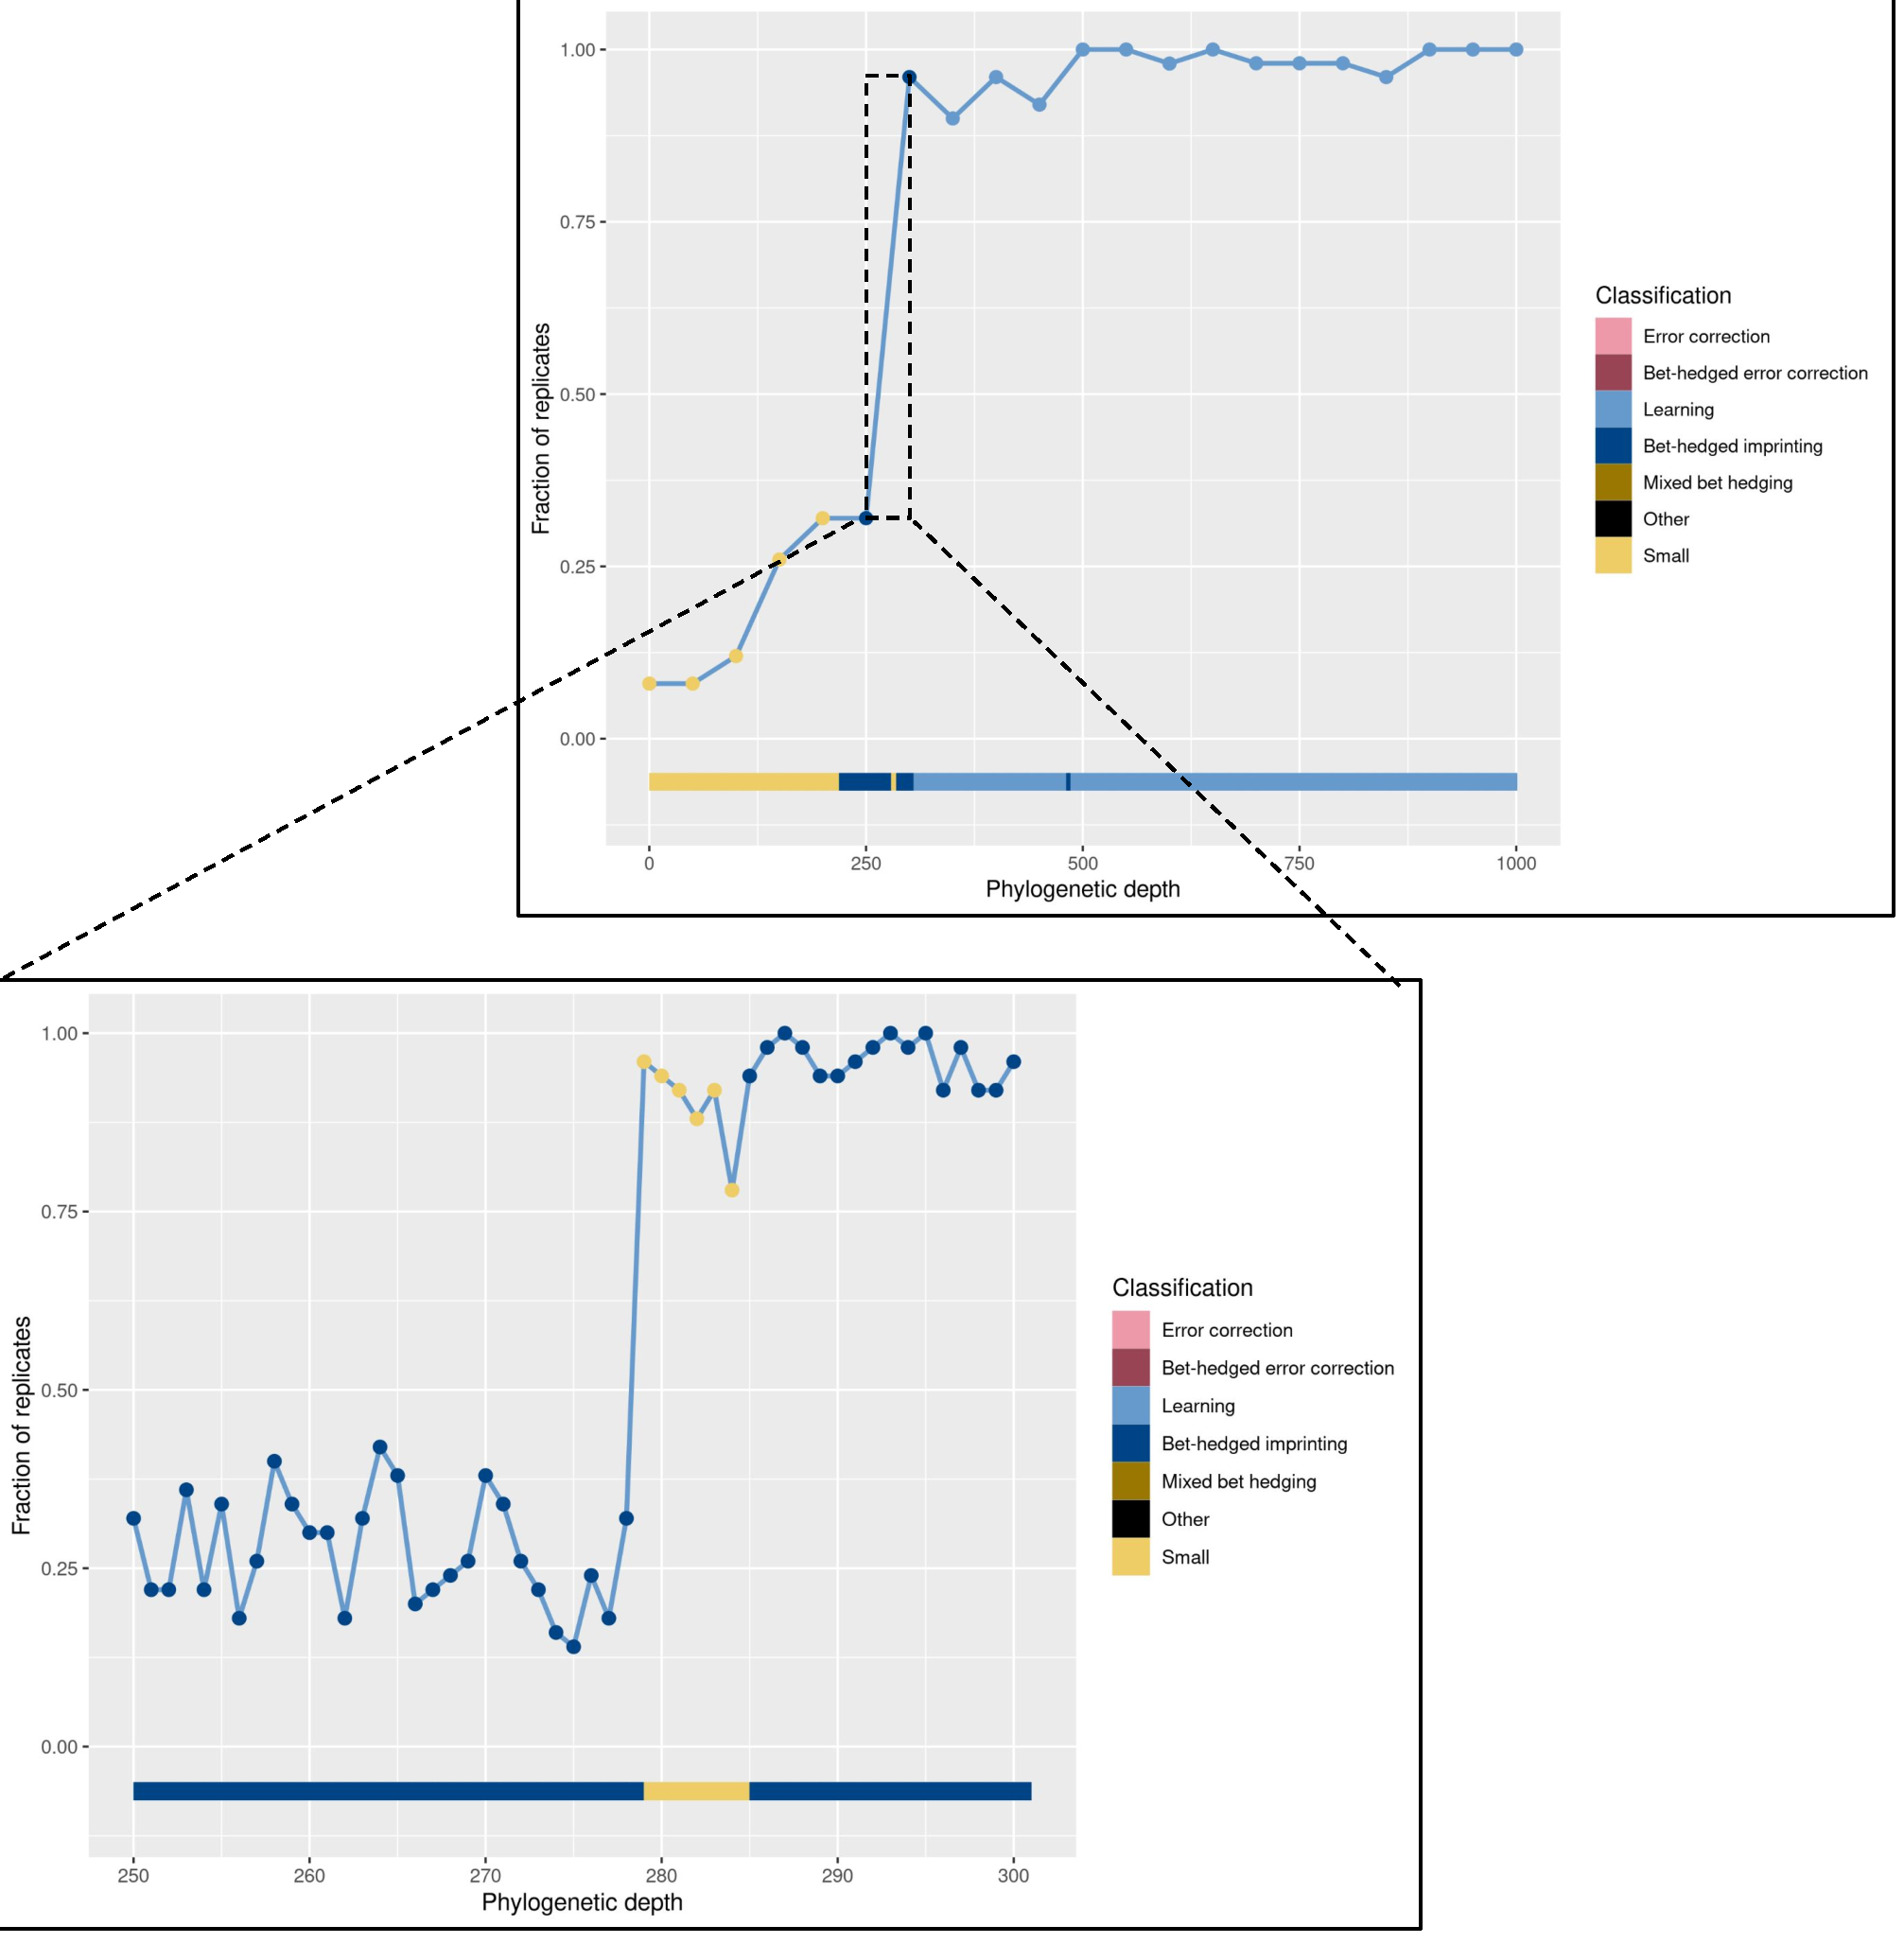
\includegraphics[width=0.45\textwidth]{media/test_pop_out_seed_15.pdf}
% \caption{
% \textbf{Case Study C}.
% Potentiation of associative learning as it changes over the lineage for Case Study C. 
% The top figure plot shows the results of the exploratory replays. 
% Two windows of increased potentiation were identified, indicated by the dashed rectangle. 
% Results of the targeted replays are shown in the bottom, pop-out plot.
% Both lines and points show potentiation at various steps along the lineage. 
% The color of the points corresponds to the behavior exhibited at that step of the lineage.
% The rectangle at the bottom of the plot also shows the behavior at the lineage, but with more detail than the evenly spaced points of the exploratory replay.}
% \label{fig-potentiation-case-study-d}
% \end{center}
% \end{figure}




\subsubsection{Lineage D}

% \begin{figure}[!h]
% \begin{center}
% 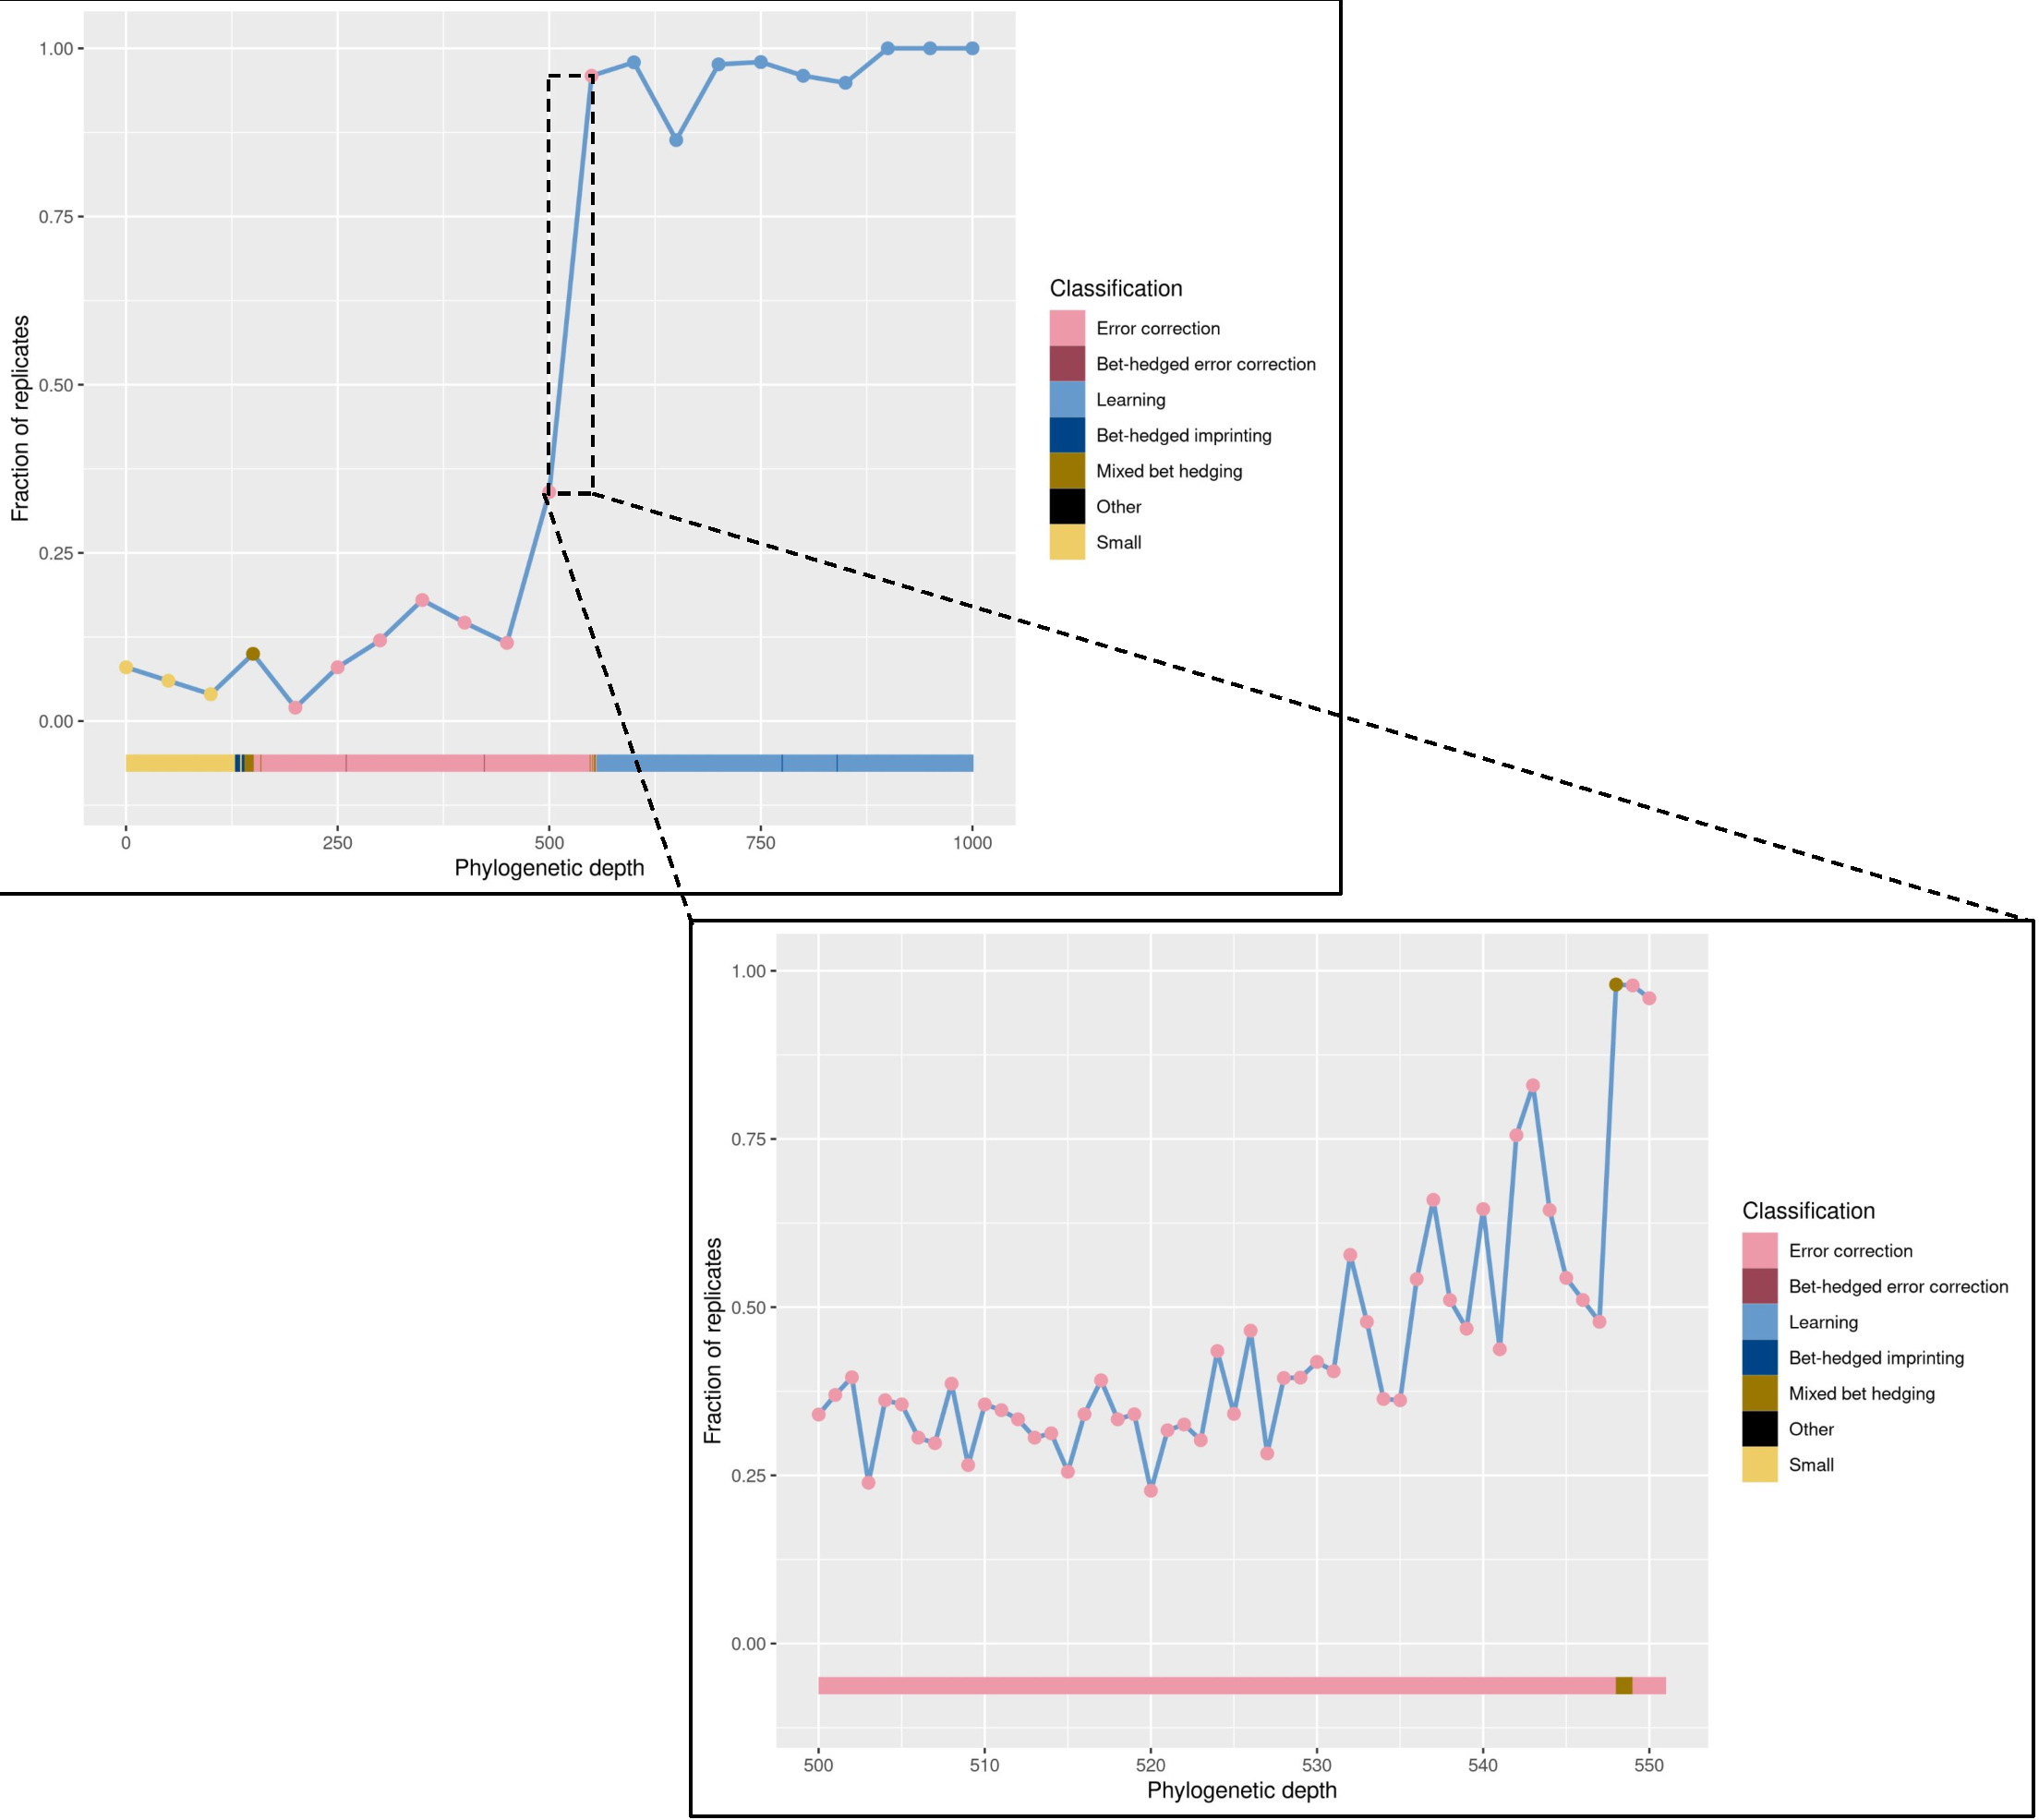
\includegraphics[width=0.45\textwidth]{media/test_pop_out_seed_6.pdf}
% \caption{
% \textbf{Case Study D}.
% Potentiation of associative learning as it changes over the lineage for Case Study D. 
% The top figure plot shows the results of the exploratory replays. 
% Two windows of increased potentiation were identified, indicated by the dashed rectangle. 
% Results of the targeted replays are shown in the bottom, pop-out plot.
% Both lines and points show potentiation at various steps along the lineage. 
% The color of the points corresponds to the behavior exhibited at that step of the lineage.
% The rectangle at the bottom of the plot also shows the behavior at the lineage, but with more detail than the evenly spaced points of the exploratory replay.}
% \label{fig-potentiation-case-study-d}
% \end{center}
% \end{figure}

Of the four replicates we analyzed, Lineage D is the only one that evolved error correction before learning.
Like the earlier lineages, the exploratory replays show that almost all potentiation comes from a single window. 
%Here, however, we only study the back half of the window, where 
In this case, potentiation grew from 34\% of replicates to 96\% between steps 500 and 550.
%Zooming in via targeted replays, potentiation in this window tells an interesting story. 
%It is hard to be certain given the noise of using 50 replay populations, but it appears that potentiation generally increases in the second half of the window. 
Targeted replays are especially noisy for this lineage, but generally show an increase in potentiation, especially in the latter half of the window.
%Of particular note are the last \~10 steps in this window. 
The largest jump in potentiation occurred at step 548, near the end of the window.
%Looking backward, however, other 
Several prior mutations also showed notable potentiation increases, but in each case later mutations appeared to counteract them. %lower potentiation again. % before later mutations lowered it again. 
Specifically, steps 542 and 543 appear to have higher potentiation than the points around them, but potentiation dipped back below 50\% before the largest jump at 548.

Out of all four lineages, D has the fewest steps between the largest potentiating step (548) and the first appearance of learning (556).
At the time, the potentiating mutations at 548 caused no discernible change in fitness even though they increased potentiation by 50 percentage points. 
Two mutations occurred at step 548: a point mutation swapped a flow control instruction for a math instruction and an insertion mutation added a comparative conditional instruction into the main execution loop. 
At step 548 the genotype encoded a naive error correction algorithm: after setup, organisms could always handle \textit{right} states, but always failed \textit{left} states, recovered, and then continued. 
%This changed when learning evolved 
%At step 556, the algorithm started sensing the environment, albeit \textit{too} often. 
A mutation at step 556 swapped a sensing instruction with a math instruction, and this combined with the prior comparison instruction from step 548 to allow the organism to move left when needed and shifted the behavior to learning.
%The organism still blundered when it encountered a state sequence of \textit{left}, \textit{forward}, \textit{left}, but it quickly recovered. 
%Since it can associate the cues with greater than 90\% accuracy, we classify it as learning. 
The local fitness landscape supports the idea that the comparison instruction was useful to the evolution of learning, as the potentiating mutation increased the number of learning genotypes in the two-step mutational neighborhood from under 800 to over 100,000.

% What's going on at 542/543?
Looking back at the apparent false start at steps 542 and 543, it is not clear what algorithmic changes these mutations conferred.
%, the potentiation mutations at steps 542 and 543 also altered 
These steps did, however, alter the set of learning behaviors that fell within the local mutational neighborhood. 
At step 541, there were only 324 two-step mutations that conferred learning, and only three of those resulted in a substantial fitness increase (a metabolic rate $> 10^{15}$). %; the merit of the best-performing mutant is ~$1.6e21$.
After steps 542 and 543, that number rose such that over 900 two-step mutations could confer learning, with over 500 resulting in a substantial fitness increase (including over 200 that reached a merit $> 10^{25}$).
We may be unsure of the exact effects of these mutations on the mechanics of the algorithm, but the changes in the local fitness landscape are profound. %to include learning algorithms with much higher fitness.


\section{Discussion and Conclusion}

%\subsection{Some mutations are potentiating.}
\subsection{Potentiation can rise suddenly}

% What evidence do we have?
We have documented several cases where single mutations dramatically increased the probability of associative learning later evolving. %arising in the longer term.
Of the four lineages analyzed, each had a single step in the lineage that resulted in a substantial increase in potentiation (ranging from 36 to 64 percentage points). 
Indeed, two of the lineages had an additional potentiating mutation that resulted in an increase of over 30 percentage points.
Looking only at exploratory replays, each lineage has a 50-step window that resulted in a potentiation increase of at least 40 percentage points.

% What does this mean?
% What does the literature say about potentiation?
While four lineages are insufficient to make any strong claims, these results demonstrate that it is \textit{possible} for single mutations to drastically increase potentiation, and provide compelling evidence that they may, in fact, be common. 
In Lineages B and D, however, we do also observe regions with smaller, incremental increases in potentiation.
Further studies are clearly necessary to more fully understand the general patterns and processes by which potentiation rises across different representations and environments.
%We do not claim that all potentiation comes from one or a few mutations, simply that future work cannot disregard the possibility that a large chunk of potentiation comes from a single mutation.


%\subsection{Some mutations are anti-potentiating.}
\subsection{Potentiation can decrease along a successful lineage}

In two of the lineages we analyzed (A and D), we see evidence of potentiation decreasing over spans of the lineage. 
%We also see mutations that decrease the probability of associative learning appearing.  
%Specifically, Lineages A and D both see jumps in potentiation that are then lost over the next section of the lineage. 
With only 50 replay populations per lineage step, our results are noisy and it is difficult to isolate what is occurring during these periods of potentiation decline.
While we were unable to identify any ``anti-potentiating'' mutations with effects as large as the positive potentiation mutations, it is possible for a single step in a lineage to greatly decrease potentiation. 

%Future work should investigate this concept of decreasing potentiation. 
Since we limited our analyses to runs where associative learning arose in the original replicate, we did not expect a preponderance of anti-potentiating mutations, but were intrigued to see evidence of them, even if at low effect.  
%However, these mutations could exist. 
These same analytic replay experiments could be applied to lineages that failed to evolve the focal behavior, to see if potentiation of that behavior experiences sudden drops. 
Similarly, our replays targeted windows with substantial increases in potentiation; other windows would be more likely to include decreases. 
Finally, failed replays from starting points with otherwise high potentiation must have failed for a reason; they too could be used as a likely source (albeit more artificial) of anti-potentiating mutations.
%Windows that see a large decrease in potentiation are more likely to contain anti-potentiating mutations, while windows of little or no potentiation change early in a lineage have the potential of an increase and subsequent decrease of potentiation within that window.
%One hypothesis is that potentiation-decreasing mutations are beneficial when they occur, and that the instant gain in fitness comes at the detriment of long-term success of evolving the complex behavior. 

%That said, in run BLAH we do see a period of steady decline in the probability of associate learning arising, though no individual mutations has a dramatic negative effect.  
%If we were to focus our replay experiments more broadly, we expect that many of the runs that never produce associative learning may exhibit more signs of anti-potentiating mutations and we plan to investigate this further in the future.

%\subsection{Potentiating mutations vary substantially from one evolutionary lineage to another}
%[Step through the different runs and talk about how different the patterns are.  Can even look at some of the runs that got associative learning, but we didn't zoom in on yet.]



\subsection{Potentiating mutations can appear innocuous when they first occur}

%[Step through these mutations and discuss how they have different immediate effects and nothing immediately identifies them as potentiating.  End with the question of "so, how are these mutations any different from other mutations?"  To have any chance of identifying potentiating mutations ahead of time, we must first further understand the underlying mechanisms that make them potentiating.]
We analyzed the mutational step in each of the four lineages that conferred the greatest increase in potentiation.
Of those four mutational events, two were neutral, one was deleterious, and one was beneficial. 
Even among these few replicates, there is no obvious pattern in the properties of potentiating mutations. 
Of the two neutral mutations, one made an instruction redundant while the other added a conditional instruction that had no effect when it was initially introduced. 
The deleterious and beneficial mutations both caused the execution flow to loop back earlier than it did before.
Additionally, the number of mutations between the potentiating mutation and the appearance of learning varied wildly between lineages, ranging from 8 steps up to 91.
The potentiating mutations in these four lineages are unique, and at the current time there is no pattern emerging among them.
So, how are these mutations any different from other mutations?
Untangling this mystery could be critical for predicting evolutionary outcomes or accelerating adaptive evolution.


% \subsection{What makes a mutation potentiating?}
\subsection{We can identify \textit{how} a mutation is potentiating}

There are many mechanisms by which a mutation could facilitate the evolution of associative learning.
For example, the mutation could provide a building block that is helpful to perform the task.  
But for a mutation to be potentiating it must notably increase the probability of associative learning appearing in the future.
Any change, no matter how helpful, that was already likely to occur would not be considered potentiating.
Indeed, it is the earlier mutations that made that change so likely that would be potentiating.
Of course, those mutations are also more challenging to identify.
%Here we define a potentiating mutation as one that increases the probability of associative learning eventually appearing by at least 0.25. (or 25 percentage points).

We have three different hypotheses for how a mutation could be potentiating:
% \begin{enumerate}
%     \item The mutation grants access to associative learning in the local fitness landscape (one or two mutations away)
%     \item Associative learning was available in the local landscape, but not beneficial; the mutation makes it valuable and drives evolution toward it.
%     \item The mutation is a ``gateway'' to another region of the fitness landscape.  It does not provide immediate access to associative learning, but it does grant access to a pathway to get there.
% \end{enumerate}
%(1) It moves through genetic space in a useful direction, providing access to associative learning in the local fitness landscape. % (one or two mutations away)
(1) It is the initial move into a genetic neighborhood with associative learning,
%(2) It improves the eventual value of associative learning, increasing the likelihood of the trait being selected if it does appear. % was available in the local landscape, but not beneficial; the mutation makes it valuable and drives evolution toward it.
%(2) It shifts toward the genetic neighborhoods of better versions of learning, improving potential fitness benefits.
(2) It is a shift into a genetic neighborhood with a more valuable version of learning, or
%(3) It is a ``gateway'' mutation to another region of the fitness landscape that does not grant immediate access to associative learning, but does unlock a pathway to get there.
%(3) It is a more general ``gateway'' mutation to another region of the fitness landscape, unlocking a pathway to learning that is undetectable using local neighborhood analyses.
(3) It is a ``gateway'' mutation that unlocks a beneficial pathway to learning, even though learning is not in the immediate genetic neighborhood.

Across the potentiating mutations we analyzed, we have found evidence for each of these hypotheses.
The largest potentiating mutation in Lineage D supports Hypothesis 1, as it is the first time in the lineage that learning is only one mutation away. 
The main potentiating mutation in Lineage A and the earlier potentiation mutations in Lineage D support Hypothesis 2 as both cause drastic increases in the fitness benefit of learning mutations in the two-step neighborhood. 
%It is worth noting that the mutation in Lineage A still only has a few two-step mutations with learning, while the mutation in Lineage D has many. 
Finally, Lineages B, C and the early potentiating mutation from Lineage A all provide support for Hypothesis 3. 
The mutations from Lineages A and B both have \textit{zero} learning mutations in their two-step neighborhoods. 
Interestingly, Lineage C sees a \textit{decrease} in the number and fitness of learning mutations in the local neighborhood. %and in the fitness of those learning mutations. 

Hypothesis 3 has many possible mechanisms by which it may work.  
For example, new traits may produce a single, clear, beneficial pathway of improvements to follow.  
Alternatively, a new building block may open a larger region with many different ways of evolving associative learning.
Finally, the mutation may actually damage existing functionality or remove existing interactions that were impeding further evolution.
While all three hypotheses have some support, future work can begin to uncover if a certain hypothesis is seen more often, what conditions might result in each scenario, or if additional analyses are needed to truly characterize these potentiating mutations. 

% Seed 86 - Hyp 2 - Increases number of two-step learning muts from 2 to 9, as well as a increase in fitness of 3 or 4 orders of magnitude
    % Seed 86 (earlier mutation) - Hyp 3 - No learning in local landscape
% Seed 4 - Hyp 3 - No learning in local landscape
% Seed 6 - Hyp 1 - Increase in the number of learning genotypes in the local neighborhood
    % Seed 6 (earlier mutations) - Hyp 2 - greatly increases the fitness benefit of learning (and maybe slightly increases the number of two-step mutations that have it)
% Seed 15 - Hyp 3 - Reduces number of learning genotypes, so not Hyp 1 or 2

\subsection{Outlook}
This work is only an early step, focused on developing techniques and expectations for performing fine-grained analyses of replay experiments. 
Next, we must expand beyond four lineages, to collect broader, more systematic replay data, automating as much of the process as possible.
%Naturally, looking at only four lineages has serious limitations, and conducting a study with enough data to aggregate the characteristics of potentiating mutations would be incredibly informative. 
We conducted this study on associative learning in Avida, but the underlying techniques must be examined broadly in other environments and substrates to ensure that our results are not unique to Avida or the evolution of associative learning. %to the specific task, so experiments that collect evidence more broadly are critical. 
Within the current study system, there are many questions that remain unanswered: 
We focused on large \textit{increases} in potentiation, but are there more obvious signals associated with \textit{decreases}?
How much of the noise that we see in our data is due to limiting ourselves to 50 replicates, and how much of it is do to actual shifts in potentiation with each mutation? % Are there signals we are missing due to noise?
What does potentiation look like in replicates that fail to evolve learning? %, or what does the potentiation of other behaviors look like in learning lineages?
%Additionally, we did not collect phylogenetic data on the replay experiments to save computational resources. 
Finally, it would be valuable to compare the specific evolutionary pathways the different replays take. Do they follow the same trend or do they differ?  This would allow us to understand if, for example, a potentiating mutation funnels evolution in a fixed direction.

Ultimately, these analytic replay techniques provide us with a tool for examining evolution in a prospective fashion, not just the retrospective approach that we are traditionally limited to.
They will allow for the development of new evolutionary theory and predictive capacity that will be invaluable, both for understanding how meaningful complexity is produced in the natural world and for improving evolutionary applications. 
        % Do this analysis, but at a scale that we can get aggregate data
        % Different substrates
        % Different tasks
        % Why only look at large _increases_ in potentiation? What's going on with the _decreases_?
        % What's going on with the lineages that _don't_ evolve learning?
        % Is sampling 50 replicates enough? 
            % Are we missing interesting trends?
            % Are we reading too much into noise?
        % We could also track phylogenies on the replays
            % How closely do replay lineages match to the original lineage?

%\section{Conclusion}

% Combined with Discussion

% \begin{figure}[t]
% \begin{center}
% \includegraphics[width=2.1in,angle=-90]{fig1.eps}
% \caption{``Energies'' (inferiorities) of strings in a first-order
%   phase transition with latent heat $\Delta\epsilon$.}
% \label{fig1}
% \end{center}
% \end{figure}

% \vspace*{-2mm}
\section{Acknowledgements}
We thank the reviewers and the MSU BEACON lab for comments. 
This work was supported by the U.S. National Science Foundation (DBI-0939454) and compute resources from the MSU Institute for Cyber-Enabled Research.

% \footnotesize
% \bibliographystyle{apalike}
% \bibliography{bibliographies/ferguson} % replace by the name of your .bib file


% \end{document}
